\documentclass[aspectratio=169]{beamer}
\usetheme{CambridgeUS}

\usepackage{graphicx} % Required for inserting images
\usepackage{amsmath, amssymb}
\usepackage{bm}
\usepackage{booktabs}
\usepackage{dsfont}
\usepackage{tikz}

\AtBeginSection[]{
  \begin{frame}
  \vfill
  \centering
  \begin{beamercolorbox}[sep=8pt,center,shadow=true,rounded=true]{title}
    \usebeamerfont{title}\insertsectionhead\par%
  \end{beamercolorbox}
  \vfill
  \end{frame}
}

%\logo{\titlegraphic{\vspace{-8.5cm}\hfill\includegraphics[width=1.5cm]{logo_polimi_scritta.eps}\hspace{0.2cm}}}

\title{Bidding on multiple advertising campaigns}
\subtitle{Online Learning Applications course project - A.Y. 2025/2026}
\author{Riccardo Piantoni}
\institute{Politecnico di Milano}
\date{\today}

\begin{document}

\begin{frame}{}
    \titlepage
\end{frame}

\begin{frame}{Outline}
    \tableofcontents
\end{frame}

\begin{frame}{But first... some definitions}
    \footnotesize
    \begin{itemize}
        \item total starting budget: $B$
        \item number of users (or, equivalently, of action rounds): $T$
        \item per-round budget: $\rho = \frac{B}{T}$
        \item set of available bids: $\mathcal{B}$
        \item bidding probability distribution over bidder actions (bids): $\gamma \in \Delta_\mathcal{B}$
        \item probability distribution of the highest competing bid of a campaign: $\mathcal{D}_m$ 
        \item utility: $f(b) = (v - b)\, \mathds{1}\left[b \ge m \right]$
        \item cost: $c(b) = b\, \mathds{1}\left[b \ge m \right]$
        \item expected utility induced by the highest competing bids probability distribution: $\bar{f}(b) = \mathbb{E}_{m \sim \mathcal{D}_m}\left[f(b) \right]$
        \item expected cost induced by the highest competing bids probability distribution: $\bar{c}(b) = \mathbb{E}_{m \sim \mathcal{D}_m}\left[c(b) \right]$
        \item expected utility induced by the bidding probability distribution: $f(\gamma) = \mathbb{E}_{b \sim \gamma}\left[f(b) \right]$
        \item expected cost induced by the bidding probability distribution: $c(\gamma) = \mathbb{E}_{b \sim \gamma}\left[c(b) \right]$
        \item overall expected utility: $\bar{f}(\gamma) = \mathbb{E}_{b \sim \gamma}\left[ \mathbb{E}_{m \sim \mathcal{D}_m}\left[(v - b)\, \mathds{1}\left[b \ge m \right] \right] \right] = \mathbb{E}_{b \sim \gamma}\left[ \mathbb{E}_{m \sim \mathcal{D}_m}\left[f(b) \right] \right]$
        \item overall expected cost: $\bar{c}(\gamma) = \mathbb{E}_{b \sim \gamma}\left[ \mathbb{E}_{m \sim \mathcal{D}_m}\left[ c(b) \right] \right] = \mathbb{E}_{b \sim \gamma}\left[ \mathbb{E}_{m \sim \mathcal{D}_m}\left[ b\, \mathds{1}\left[b \ge m \right] \right] \right]$
    \end{itemize}
\end{frame}

\section{Requirement 1: stochastic single-campaign environment}

% ============================================================
% Overview
% ============================================================
\begin{frame}{Stochastic single-campaign environment}
    \begin{itemize}
        \item One campaign, $T$ sequential first-price auctions
        \item Stochastic environment = stationary stochastic process, with a constant-across-rounds distribution $\mathcal{D}_m$ of the highest competing bid $m$ (unknown by the bidder)
        \item Per-round budget $\rho = B/T$, total budget $B$ (possibly $+\infty$ to model no-budget setting)
        \item Valuation $v$ of the bidder
        \item Two settings to be studied:
        \begin{itemize}
            \item \textbf{UCB-like} without budget
            \item \textbf{UCB-like} with budget
        \end{itemize}
    \end{itemize}
\end{frame}

% ============================================================
% Competing-bid distribution
% ============================================================
\begin{frame}{Competing-bid distribution: from uniform to Beta}
    % \begin{columns}[T]
    %     \begin{column}{0.5\textwidth}
    %         \textbf{Modeling choice.}
    %         \begin{itemize}
    %             \item $n$ competitors draw bids $X_i \sim \mathrm{Unif}(0,1)$
    %             \item Maximum $m = \max_i X_i \sim \mathrm{Beta}(n, 1)$
    %             \item Win probability $P(b \ge m) = b^n$
    %             \item $\Rightarrow$ classical stochastic bandit on $b \in [0,1]$ with unknown $n$
    %         \end{itemize}
    %     \end{column}
    %     \begin{column}{0.5\textwidth}
    %         \centering
    %         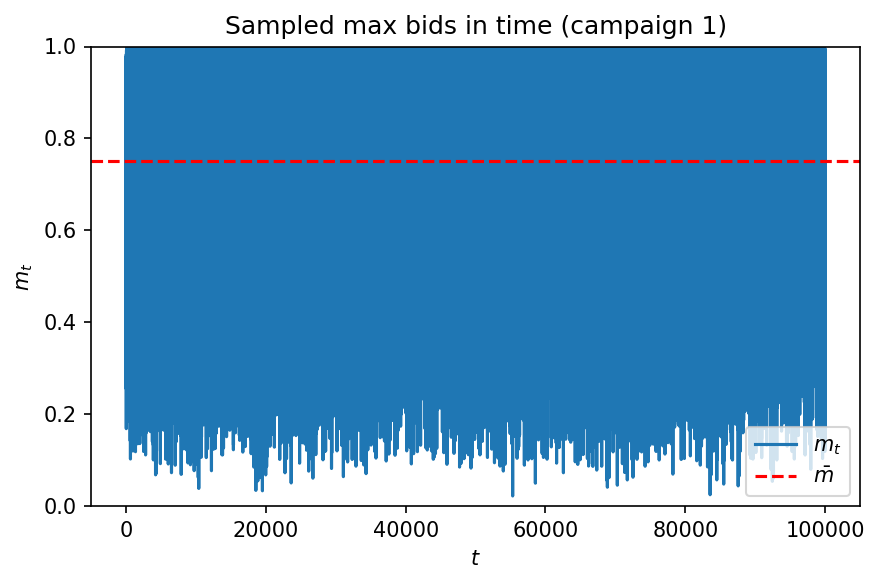
\includegraphics[width=\textwidth]{figures/req1_max_bids_ts.png}\\
    %         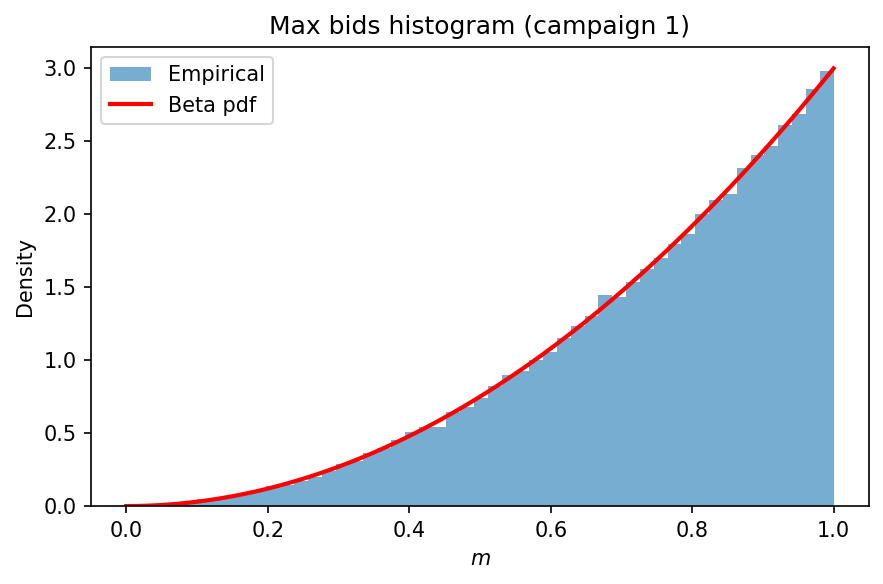
\includegraphics[width=\textwidth]{figures/req1_max_bids_hist.png}
    %     \end{column}
    % \end{columns}

    \textbf{Modeling choice:}
    \begin{columns}[T]
        \begin{column}{0.5\textwidth}
            \begin{itemize}
                \item $n$ competitors draw bids $X_i \sim \mathrm{Unif}(0,1)$
                \item Maximum $m = \max_i X_i \sim \mathrm{Beta}(n, 1)$
            \end{itemize}
        \end{column}
        \begin{column}{0.5\textwidth}
             \begin{itemize}
                \item PDF: $\mathbb{P}\left[ m = b \right] = n b^{n-1}$
                \item CDF (win probability): $\mathbb{P}\left[ m \le b \right] = b^n$
            \end{itemize}
        \end{column}
    \end{columns}
    \vspace{0.5cm}
    \centering
    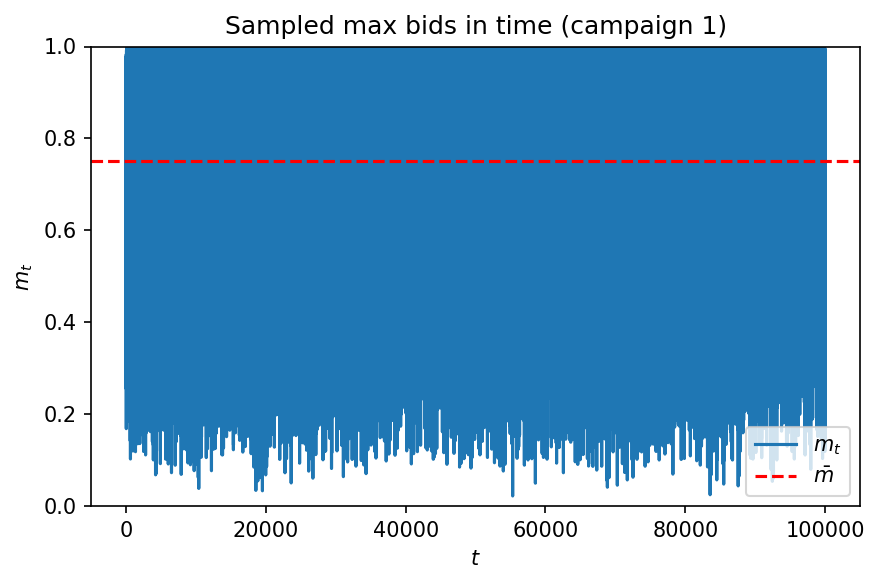
\includegraphics[width=0.4\textwidth]{figures/req1_max_bids_ts.png}
    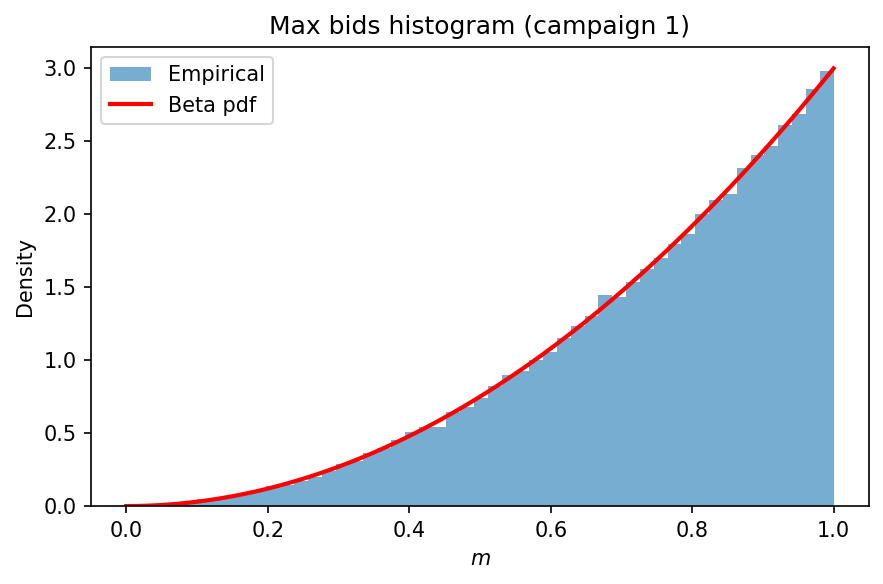
\includegraphics[width=0.4\textwidth]{figures/req1_max_bids_hist.png}
\end{frame}

% ============================================================
% Clairvoyant LP
% ============================================================
\begin{frame}{Clairvoyant}
    A clairvoyant "in expectation":
    \begin{itemize}
        \item the highest competing bids $m_t$ are stochastic and sampled from a distribution $\mathcal{D}_m$ \\
        $\implies$ we need the best behavior \emph{on average}
        \item the clairvoyant only needs to satisfy the budget constraint \emph{in expectation}, but is allowed to exceed per-round budget at any round
    \end{itemize}
    
    \begin{block}{Assumption} 
    The clairvoyant knows the underlying distribution $\mathcal{D}_m$ of the highest competing bids $m_t$, but not their actual realizations!
    \end{block}
\end{frame}

\begin{frame}{Clairvoyant - example}
    Consider the following simple setting:
    \begin{itemize}
        \item discretized bids space $\mathcal{B} = \{0.0, 0.4\}$
        \item ad valuation of the bidder $v = 0.8 \implies$ if you win, you always get a reward
        \item per-round budget $\rho = 0.2$
        \item expected highest competing bid $\mathbb{E}_{m \sim \mathcal{D}_m}\left[m\right] = 0.1$
    \end{itemize}   
\end{frame}

\begin{frame}{Clairvoyant - example}
    In this setting:
    \begin{itemize}
        \item always bidding 0.0 respects the budget constraint but never wins any auction and thus never gets any value ($f = 0.0$)
        \item always bidding 0.4 gets some value, but will likely exceed the budget constraint in expectation
    \end{itemize}

    $\implies$ a distribution over bids is needed!

    \begin{block}{} 
        There exists a single optimal bid (by existence of a deterministic policy in a stationary MDP), but we cannot use it because of the discretization of the bids space!
    \end{block}
\end{frame}

\begin{frame}{Clairvoyant - definition}
    Choose an optimal \emph{distribution} $\gamma^\star(b)$ over bids that:
    \begin{columns}[T]
        \begin{column}{0.5\textwidth}
            \centering
            maximizes the final expected reward
        \end{column}
        \begin{column}{0.5\textwidth}
            \centering
            subject to the budget constraint in expectation
        \end{column}
    \end{columns}

    \vspace{-0.2cm}
    
    \small\begin{equation*}
        \begin{aligned}
            \gamma^\star &= \arg \max_{\gamma \in \Delta_\mathcal{B}} ~~~ \bar{f}(\gamma) \qquad \qquad \qquad \qquad \qquad \qquad \qquad & \text{s.t.  } T \bar{c}(\gamma) \le B \\
            &= \arg \max_{\gamma \in \Delta_\mathcal{B}} ~~~ \bar{f}(\gamma) & \text{s.t.  } \bar{c}(\gamma) \le \rho \\    
            &= \arg \max_{\gamma \in \Delta_\mathcal{B}} ~~~ \mathbb{E}_{b \sim \gamma}\left[ \mathbb{E}_{f \sim \mathcal{D}}\left[ f(b) \right] \right] & \text{s.t.  } \mathbb{E}_{b \sim \gamma}\left[ \mathbb{E}_{c \sim \mathcal{D}}\left[ c(b) \right] \right] \le \rho \\
            &= \arg \max_{\gamma \in \Delta_\mathcal{B}} ~~~ \mathbb{E}_{b \sim \gamma}\left[ \mathbb{E}_{m \sim \mathcal{D}_m}\left[(v - b)\, \mathds{1}\left[b \ge m \right] \right] \right] & \text{s.t.  } \mathbb{E}_{b \sim \gamma}\left[ \mathbb{E}_{m \sim \mathcal{D}_m}\left[ b\, \mathds{1}\left[b \ge m \right] \right] \right] \le \rho \\    
            &= \arg \max_{\gamma \in \Delta_\mathcal{B}} ~~~ \mathbb{E}_{b \sim \gamma}\left[(v - b)\, \mathbb{E}_{m \sim \mathcal{D}_m}\left[\mathds{1}\left[ b \ge m \right] \right] \right] & \text{s.t.  } \mathbb{E}_{b \sim \gamma}\left[b\, \mathbb{E}_{m \sim \mathcal{D}_m}\left[ \mathds{1}\left[b \ge m \right] \right] \right] \le \rho \\    
            &= \arg \max_{\gamma \in \Delta_\mathcal{B}} ~~~ \mathbb{E}_{b \sim \gamma}\left[(v - b)\, \mathbb{P}_{m \sim \mathcal{D}_m}\left[b \ge m \right] \right] & \text{s.t.  } \mathbb{E}_{b \sim \gamma}\left[b\, \mathbb{P}_{m \sim \mathcal{D}_m}\left[b \ge m \right] \right] \le \rho \\    
            &= \arg \max_{\gamma \in \Delta_\mathcal{B}} ~~~ \sum_b \gamma(b)\, \underbrace{(v - b)\, \mathbb{P}_{m \sim \mathcal{D}_m} \left[b \ge m \right]}_{\bar{f}(b)} & \text{s.t.} \sum_b \gamma(b)\, \underbrace{b\, \mathbb{P}_{m \sim \mathcal{D}_m}\left[b \ge m \right]}_{\bar{c}(b)} \le \rho
        \end{aligned}
    \end{equation*}
\end{frame}

\begin{frame}{Clairvoyant - Linear Program}
    By writing the simplex constraints explicitly, we obtain the following Linear Program (LP): 
    
    \begin{equation*}
        \begin{aligned}
            \gamma^\star = \arg & \max_{\gamma \in \mathbb{R}^K} ~~~ \sum_b \gamma(b)\, \bar{f}(b) \\
            & \begin{aligned} 
                \text{s.t.} ~~~~~~ & \sum_b \gamma(b)\, \bar{c}(b) \le \rho \\
                & \sum_b \gamma(b) = 1 \\
                & 0 \le \gamma(b) \le 1\quad \forall b 
            \end{aligned}
        \end{aligned}
    \end{equation*}
\end{frame}

\begin{frame}{Clairvoyant - optimal distribution $\gamma^\star$ over bids}
    \begin{itemize}
        \item With budget, $\gamma^\star$ can concentrate on multiple bids, attempting to spend exactly the whole available budget
        \item \textbf{Note:} for $B = +\infty$ the budget constraint disappears $\implies$ we no longer care about the cost and can choose whatever deterministic bid we want, even if we overspend
    \end{itemize}
        
    \centering
    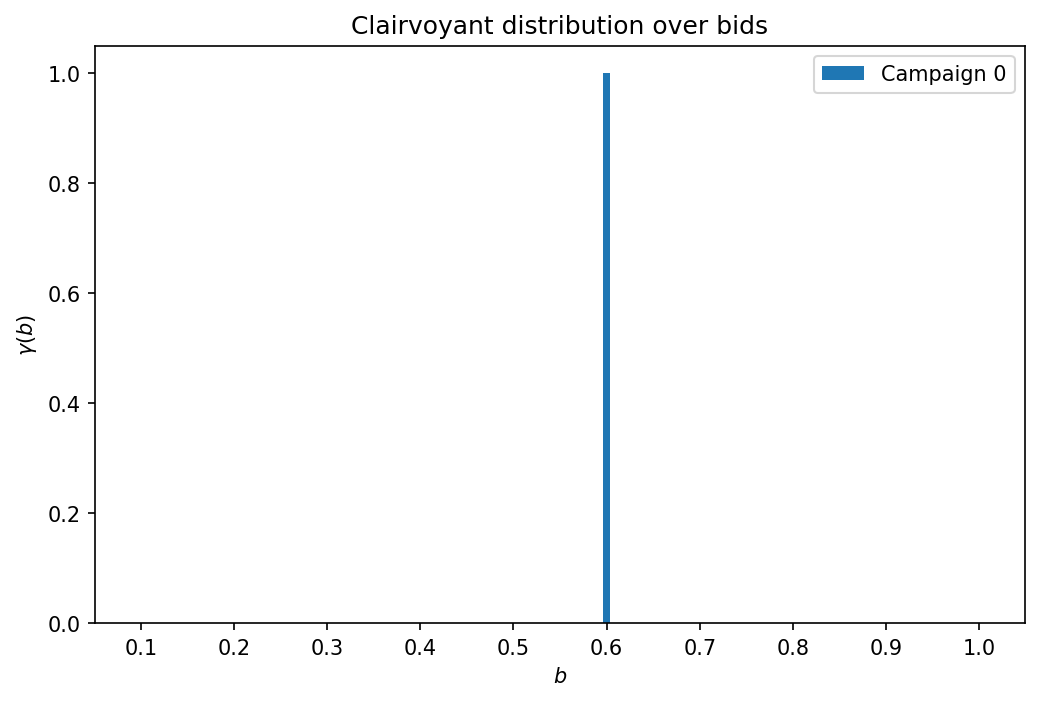
\includegraphics[width=0.35\textwidth]{figures/req1_clairvoyant_gamma_no_budget.png}
    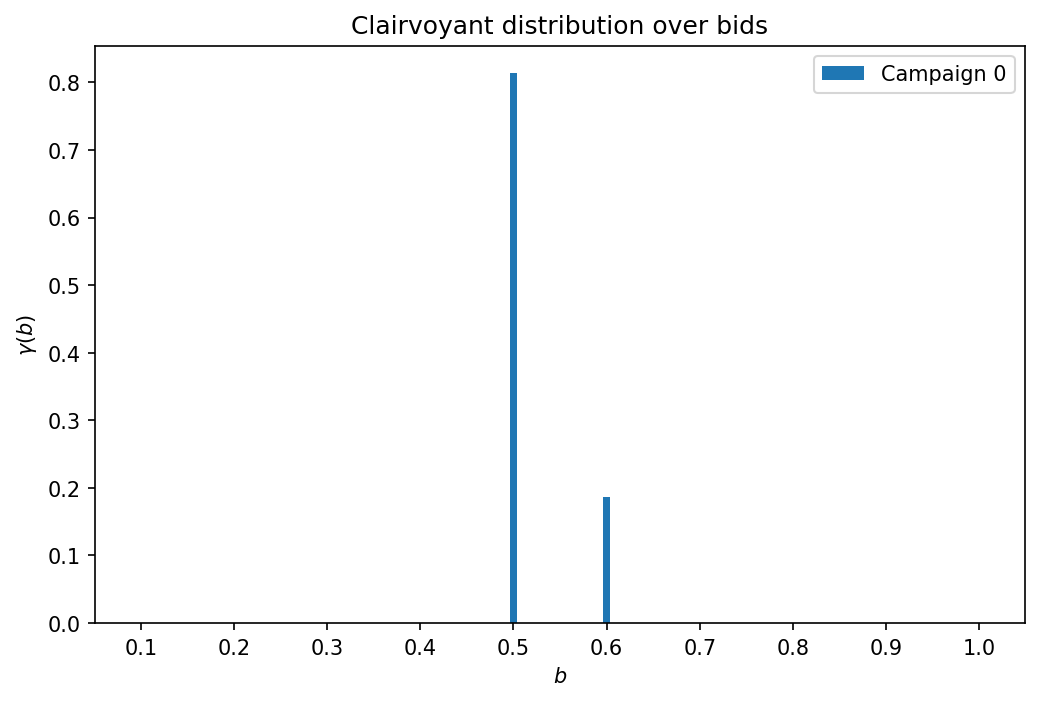
\includegraphics[width=0.35\textwidth]{figures/req1_clairvoyant_gamma_budget.png} \\
    \scriptsize
    \textbf{Left:} with no budget, the LP puts all the probability mass on the bid $b^\star$ that maximizes $\bar{f}(b) = (v - b)\,\mathbb{P}(b\ge m)$ \\ \textbf{Right:} with budget, it splits the probability mass on two adjacent bids
\end{frame}

% ============================================================
% UCB-like bidder
% ============================================================
\begin{frame}{UCB-like bidder: algorithm}
    \begin{itemize}
        \item Treat each bid $b \in \{0, 0.1, \dots, 1.0\}$ as an arm
        \item Keep track of empirical means $\hat{f}(b)$, $\hat{c}(b)$ from bandit feedback
        \item Compute the current confidence radius: \[r(b) = v \cdot \sqrt{\frac{2 \log t}{N(b)}}\]
        \item Use it to implement optimism: \[\hat{f}_{\mathrm{UCB}}(b) = \min\{\hat{f}(b)+r(b), 1\},\] \[\hat{c}_{\mathrm{LCB}}(b) = \max\{\hat{c}(b)-r(b), 0\}\]
    \end{itemize}
\end{frame}

\begin{frame}{UCB-like bidder: action selection}
    \begin{itemize}
        \item \textbf{Exploration rounds (first $K$ rounds):}  round-robin exploration of all the $K$ bids
        \item \textbf{Action selection:} we can solve the same LP as the clairvoyant, replacing the true $\bar{f}(b)$ and $\hat{c}(b)$ with the optimistic estimates
        \begin{equation*}
            \begin{aligned}
                \gamma^\star = \arg & \max_{\gamma \in \mathbb{R}^K} ~~~ \sum_b \gamma(b)\, \hat{f}_{\mathrm{UCB}} \\
                & \begin{aligned} 
                    \text{s.t.} ~~~~~~ & \sum_b \gamma(b)\, \hat{c}_{\mathrm{LCB}} \le \rho, \\
                    & \sum_b \gamma(b) = 1 \\
                    & 0 \le \gamma(b) \le 1\quad \forall b 
                \end{aligned}
            \end{aligned}
        \end{equation*}
        and then sample a bid from the resulting optimal distribution $\gamma^\star$
    \end{itemize}
\end{frame}

% ============================================================
% No-budget vs Budget comparison
% ============================================================

\begin{frame}{No-budget: empirical behavior}
    \begin{columns}[T]
        \begin{column}{0.5\textwidth}
            \centering
            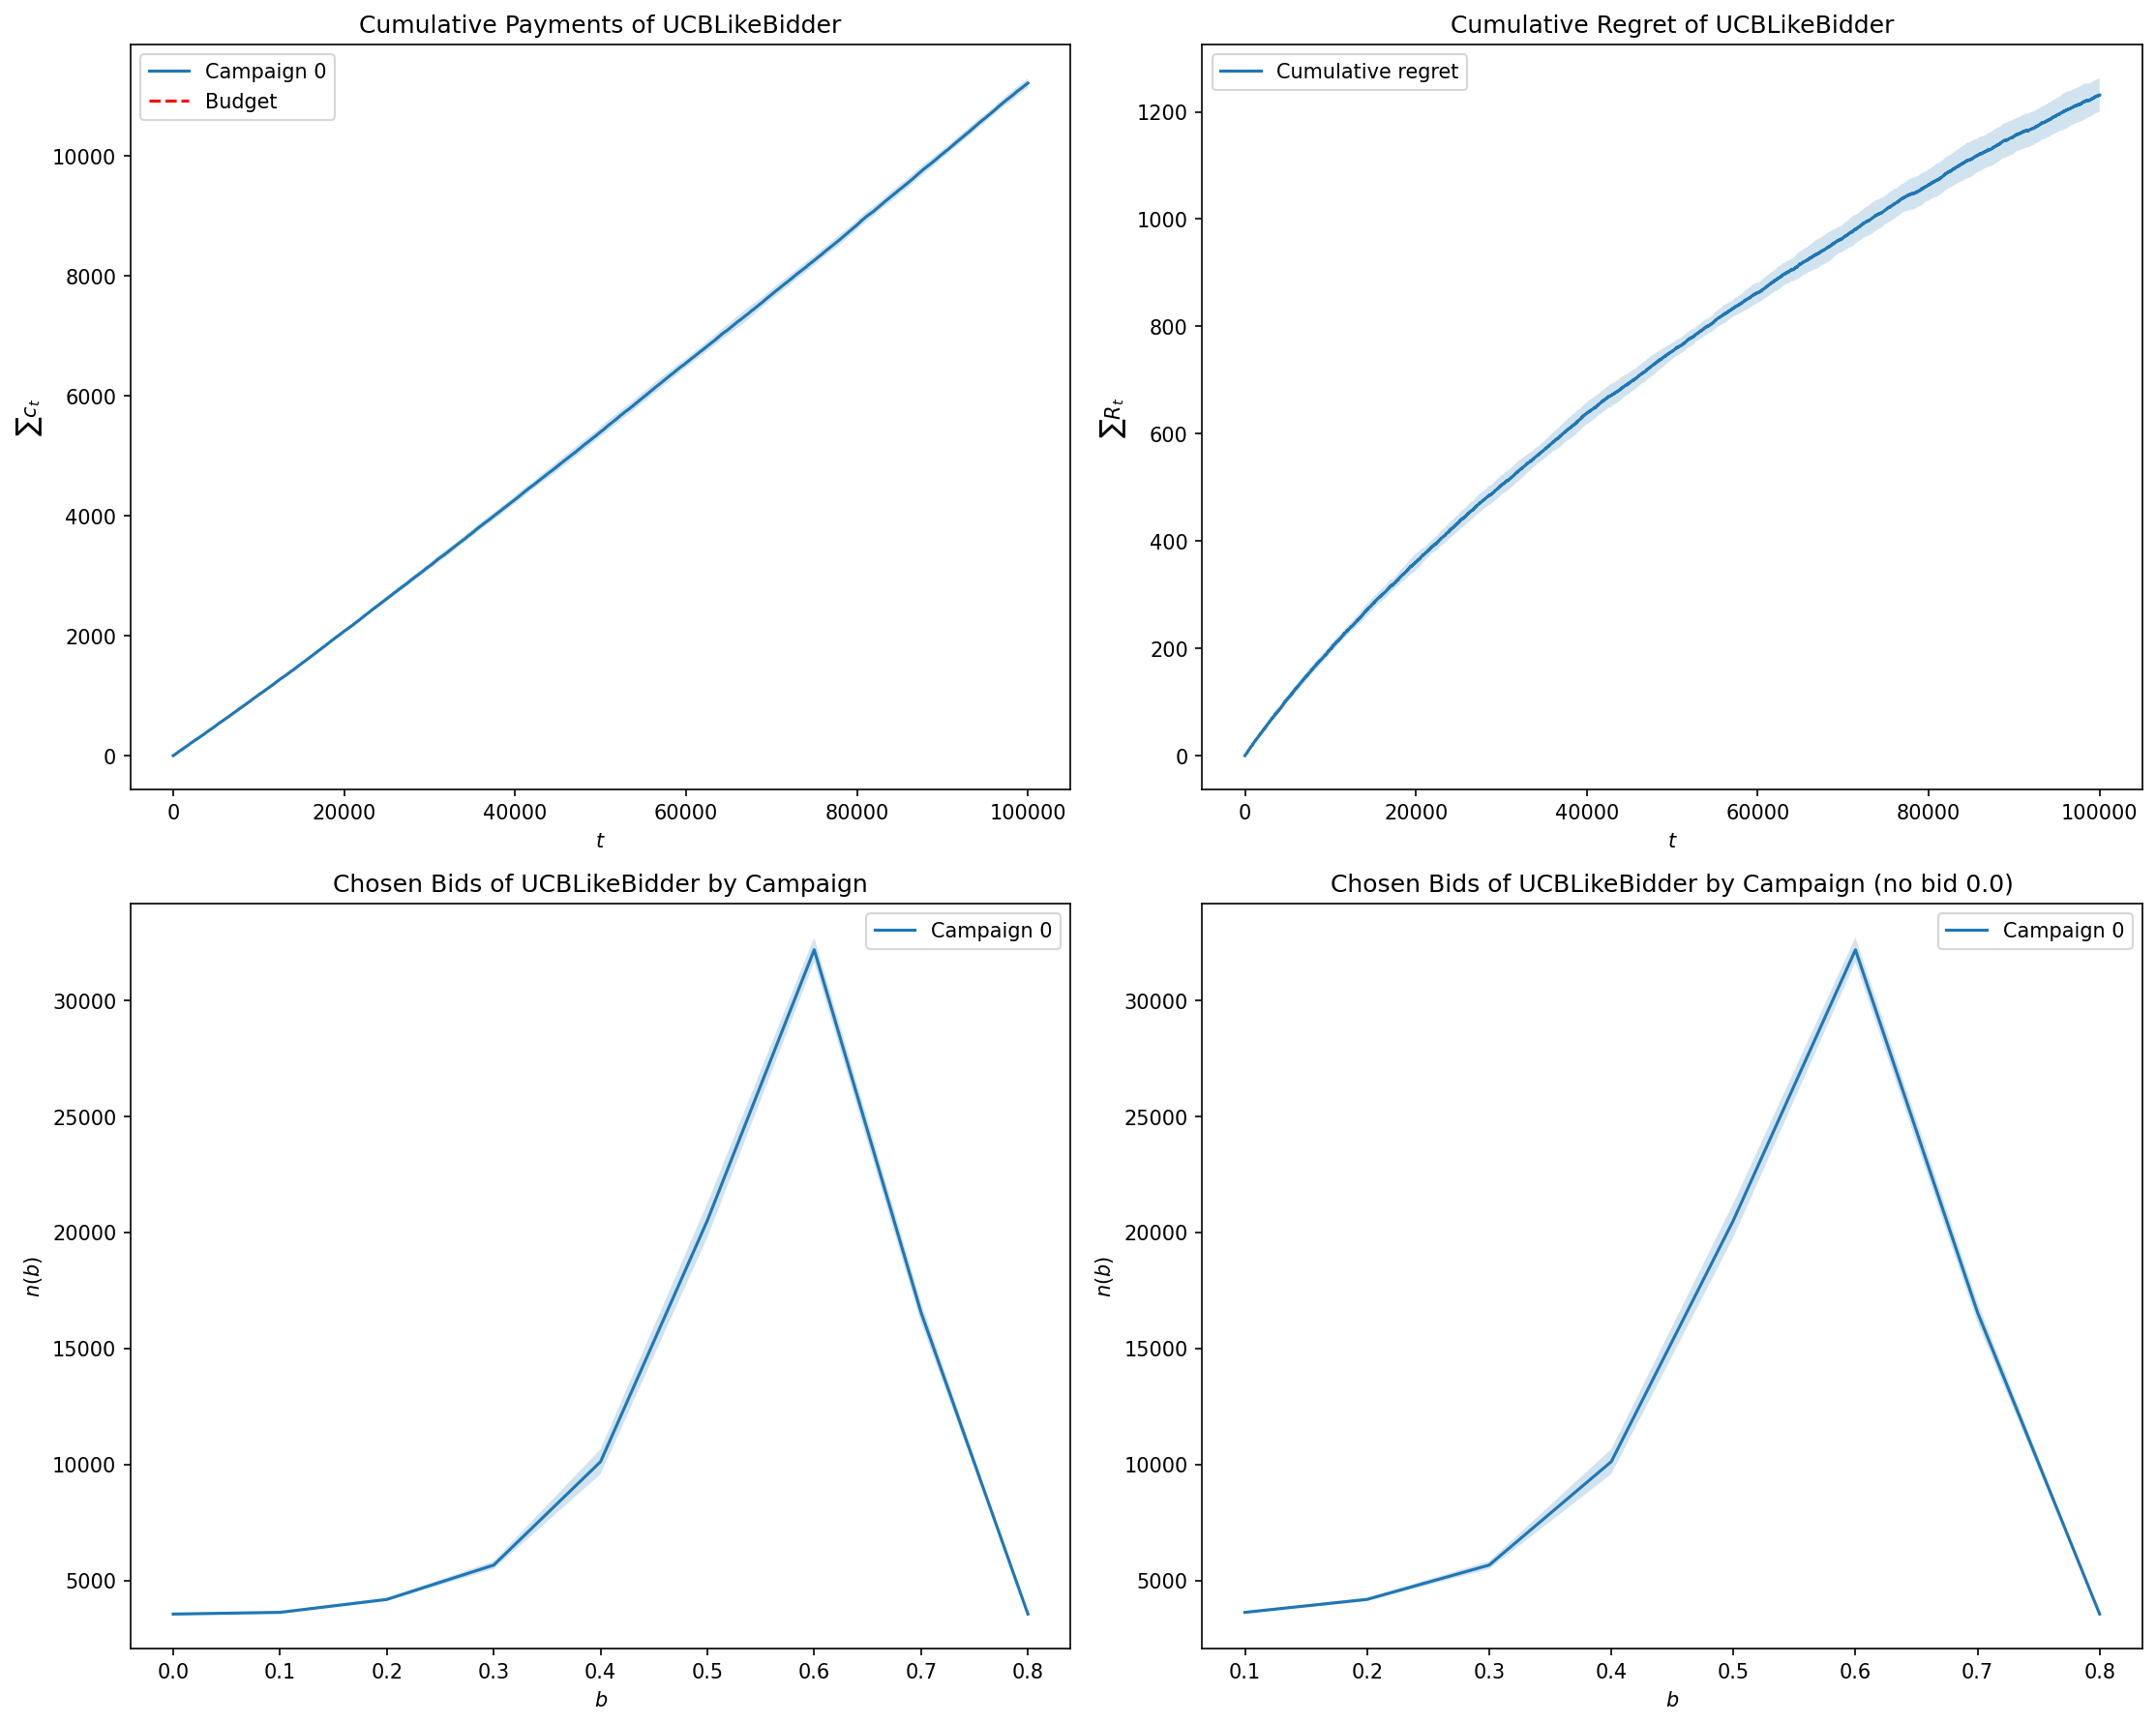
\includegraphics[width=0.95\textwidth]{figures/req1_no_budget_experiment_results.png}
            \scriptsize
            \textbf{$\rho = \infty$:} bid mass concentrates on the single arm maximizing $f_{\mathrm{UCB}}$ (matches the no-budget clairvoyant).
        \end{column}
        \begin{column}{0.5\textwidth}
             \begin{itemize}
                \item It takes $100000$ (!) rounds for the UCB-like bidder to start exhibiting sublinear regret
                \item This is because the confidence radius decay slowly for an action space of $|\mathcal{B}| = 10$ bids $\implies$ a confidence radius that decays faster should be studied 
                \item Still, the played bids are concentrating around the bid played by the no-budget clairvoyant
            \end{itemize}
        \end{column}
    \end{columns}
\end{frame}

\begin{frame}{Budget: empirical behavior}
    \begin{columns}[T]
        \begin{column}{0.5\textwidth}
            \centering
            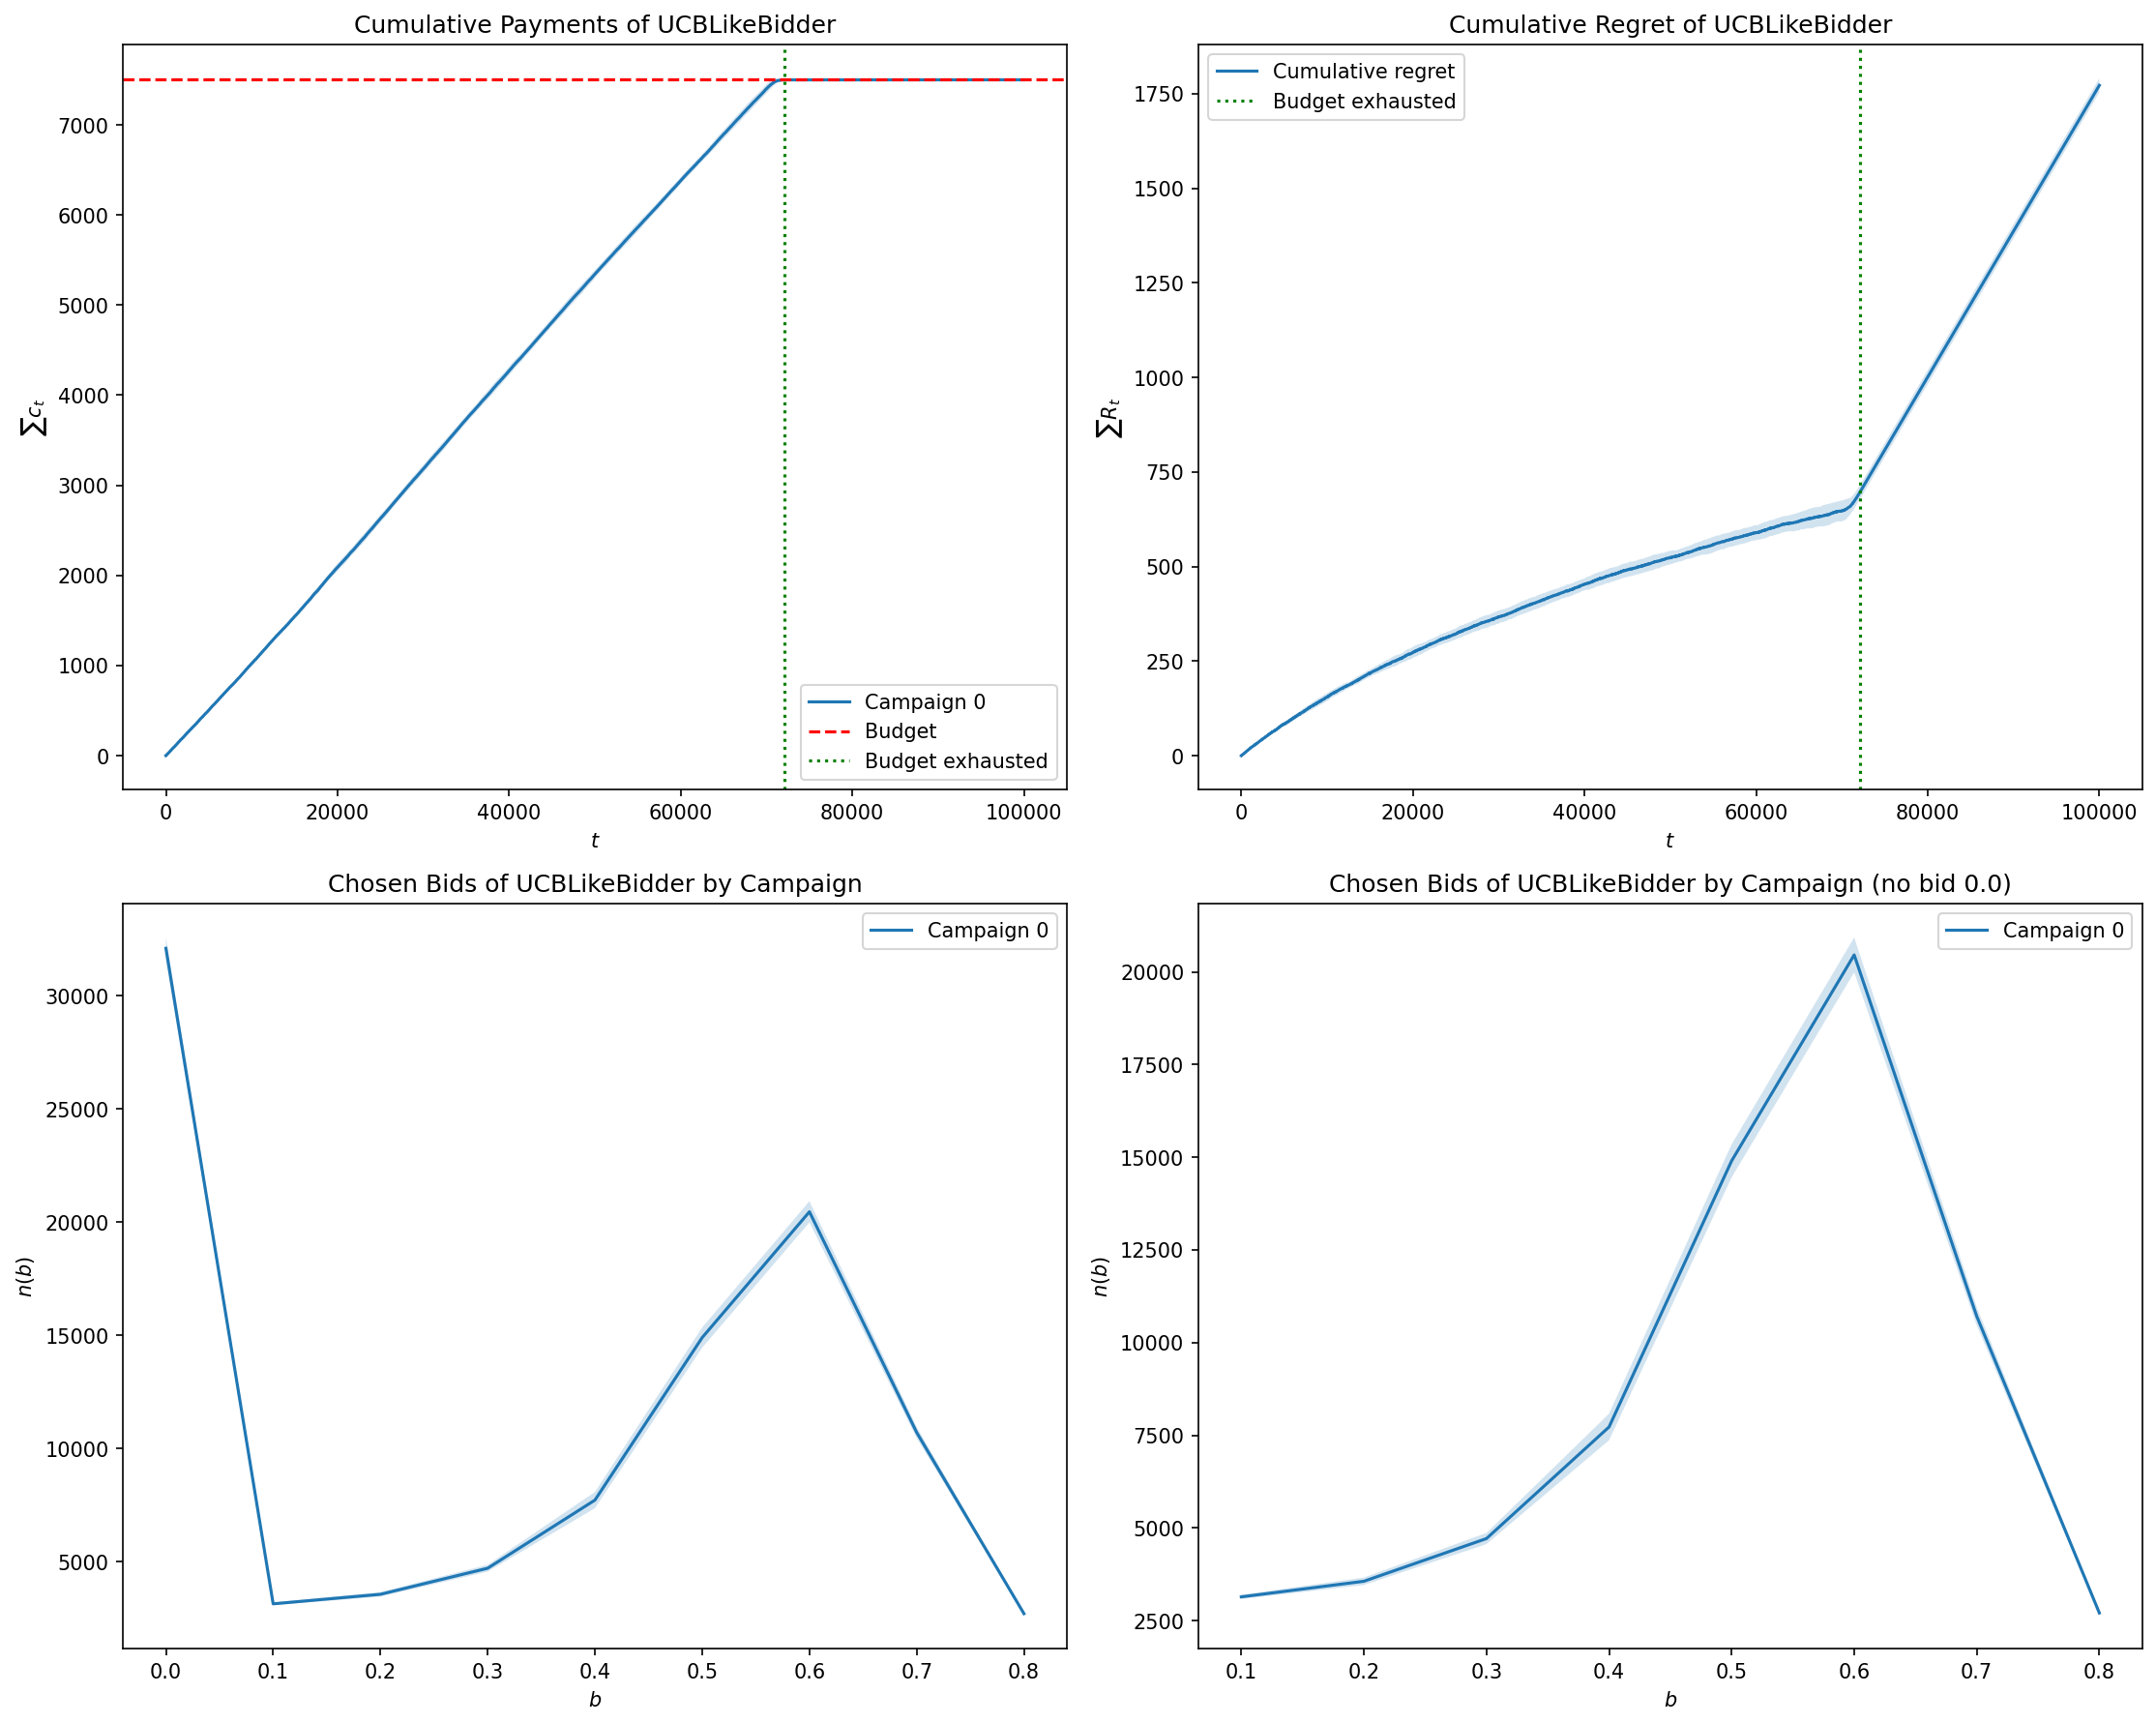
\includegraphics[width=0.95\textwidth]{figures/req1_budget_constrained_experiment_results.png}
            \scriptsize
            \textbf{$\rho < \infty$:} there are a lot of no-bid actions, because the budget gets depleted. Also, other bids are more spread out
        \end{column}
        \begin{column}{0.5\textwidth}
             \begin{itemize}
                \item Again, sublinear regret after a lot of rounds
                \item The peak in the played action is also once again concentrating around the bids played by the no-budget clairvoyant
            \end{itemize}
        \end{column}
    \end{columns}
\end{frame}

\begin{frame}{No-budget vs budget: regret comparison}
    \centering
    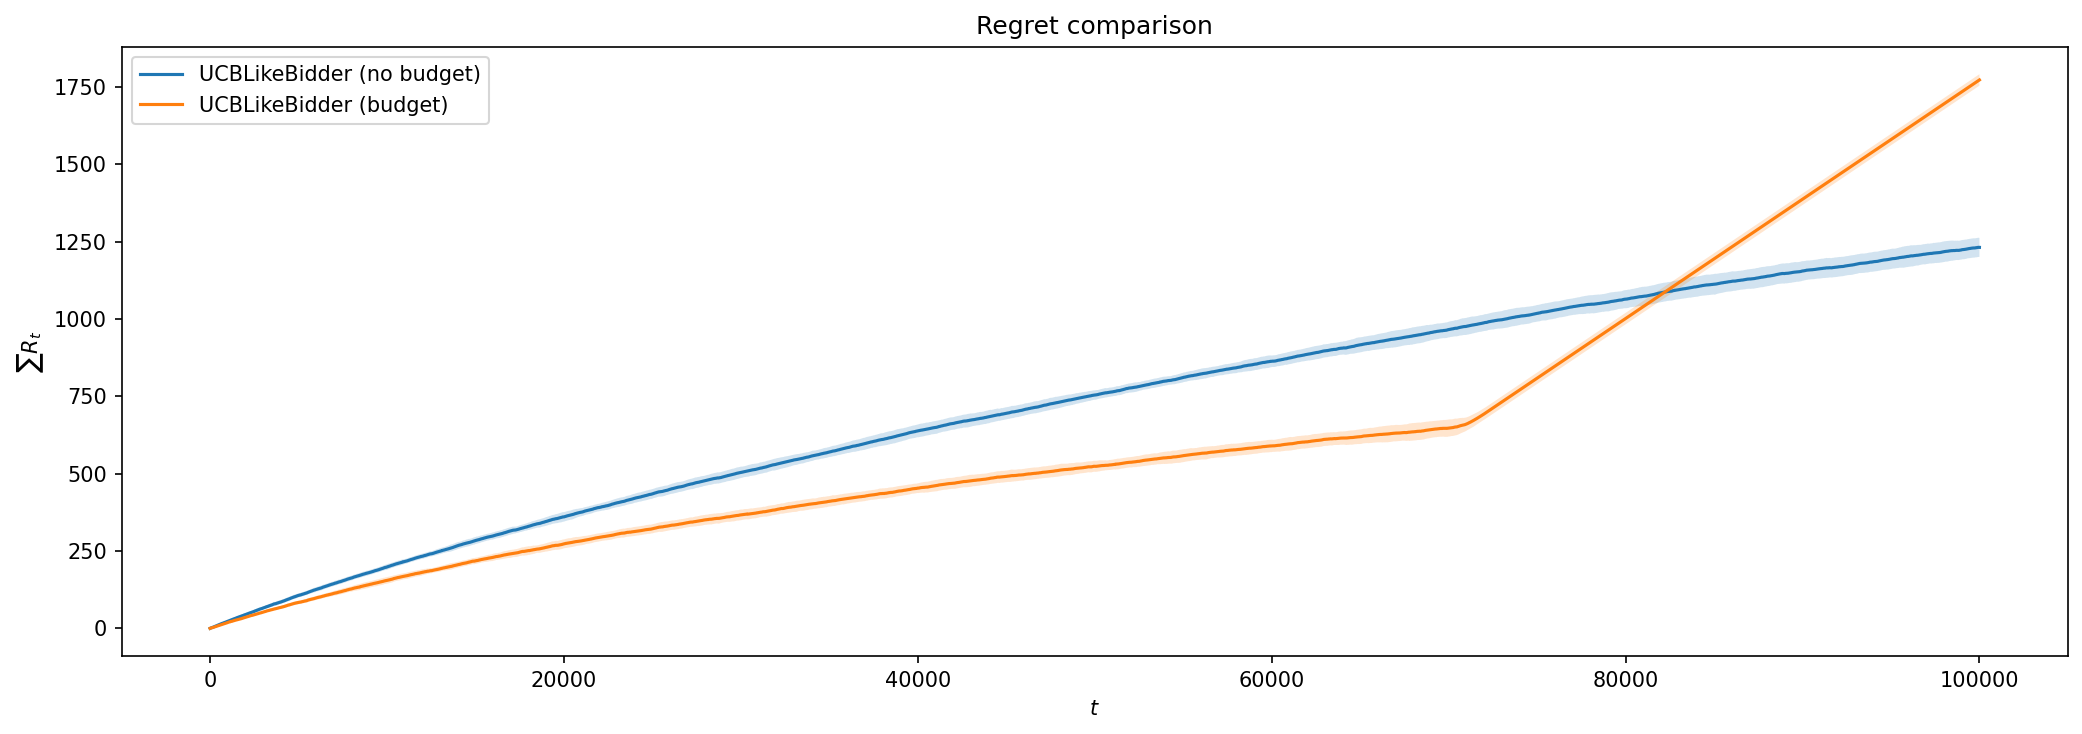
\includegraphics[width=0.9\textwidth]{figures/req1_regret_compare.png}\\
    \scriptsize
    Sublinear regret in both regimes. \textcolor{orange}{With budget}, regret is initially lower because the clairvoyant utility itself is restricted by the budget constraint; however, it eventually skyrockets when the budget is depleted, while the \textcolor{blue}{no-budget} regret keeps growing with a sublinear trend.
\end{frame}

\begin{frame}{Budget pacing}
    \centering
    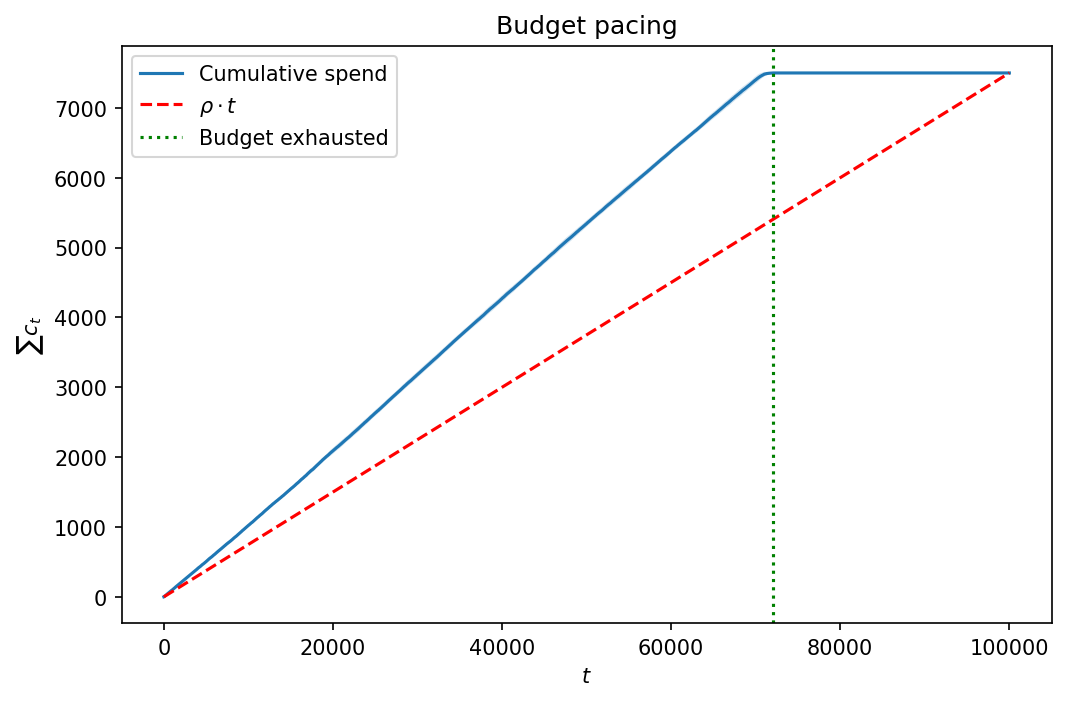
\includegraphics[width=0.37\textwidth]{figures/req1_budget_pacing.png}\hfill
    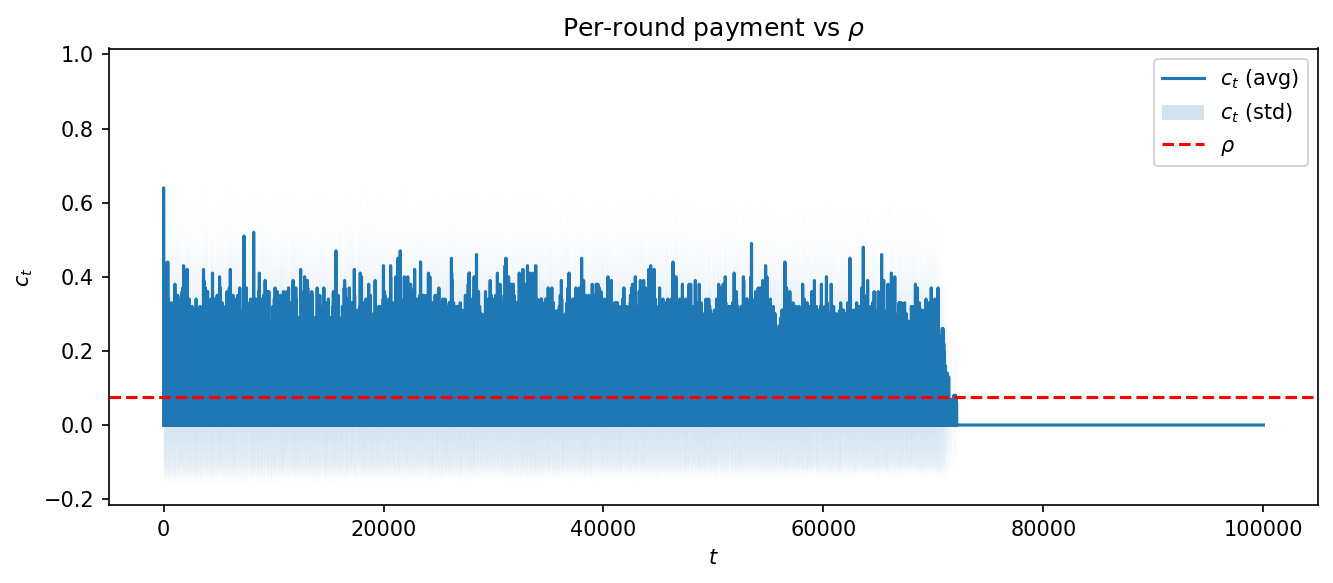
\includegraphics[width=0.57\textwidth]{figures/req1_per_round_payment_vs_rho.png}\\
    \scriptsize
    In the budget-constrained setting, we observe the bidder overspending (\textbf{left plot)}) with respect to the per-round budget $\rho$: this is likely because of exploration, as it seems to be possible to spend much more than $\rho$, while it is not possible to spend that much less (\textbf{right plot)}). 
\end{frame}


\section{Requirement 2: stochastic multiple-campaigns environment}

% ============================================================
% Overview
% ============================================================
\begin{frame}{Stochastic multiple-campaigns environment}
    \begin{itemize}
        \item $N$ campaigns, each with its own ad valuation $v^{(i)}$, and joint highest-bid distribution $\mathcal{D}_{\mathbf{m}}$
        \item Single shared budget $B$ across \emph{all} campaigns
        \item Conflict graph $\mathcal{G}$: certain pairs of campaigns are mutually exclusive (cannot win both)
        \item Action per round: choose $N$ bids, one for each campaign, from a bid space $\mathcal{B}$ of size $K$ $\implies K^N$ possible superarms
        \item Algorithm to be studied: \textbf{Combinatorial-UCB} with budget
        \begin{itemize}
            \item Its output is a distribution $\gamma$ for the probability of choosing each superarm
        \end{itemize}
    \end{itemize}
\end{frame}

% ============================================================
% Conflicts graph
% ============================================================

\begin{frame}{Conflict graph - model}
    A graph in which:
    \begin{itemize}
        \item each node represents a campaign
        \item an edge between two nodes represents a conflict between incompatible campaigns, meaning that they cannot be bid on during the same round (but both can be bid on in different rounds)
    \end{itemize}

    \centering
    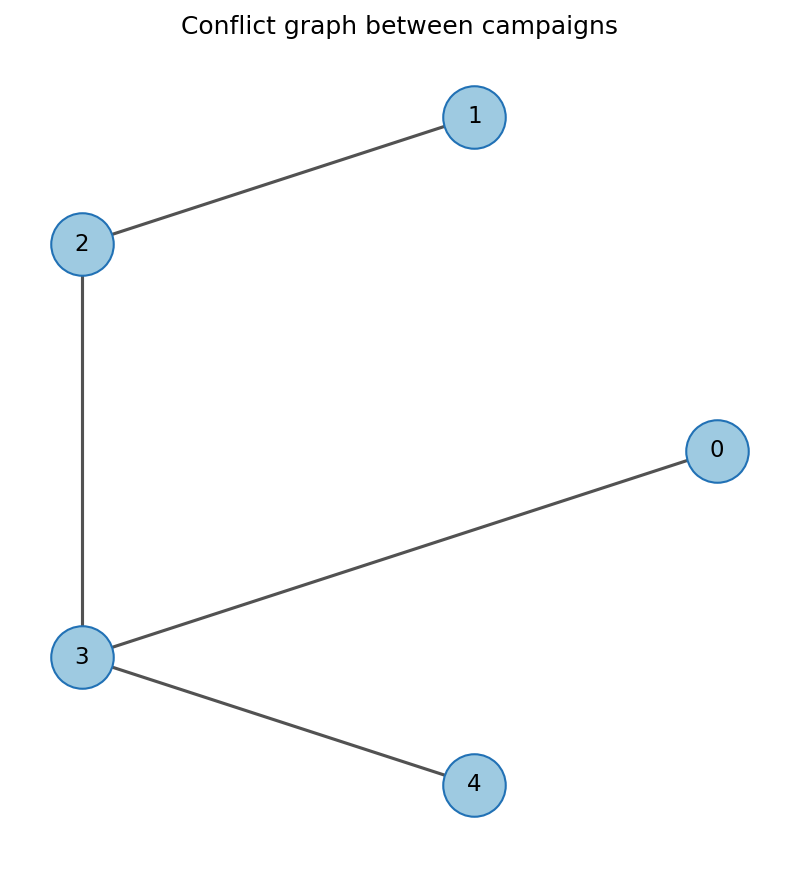
\includegraphics[width=0.26\textwidth]{figures/req2_conflict_graph.png} $\qquad$
    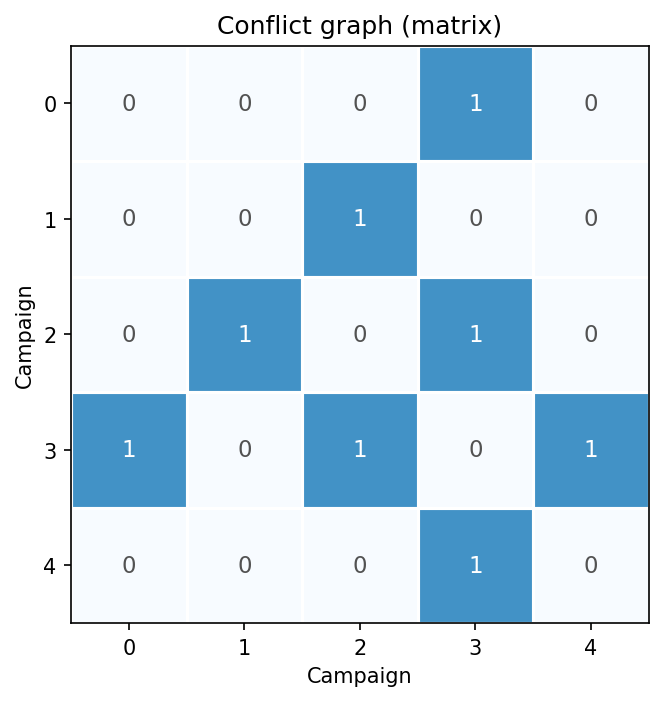
\includegraphics[width=0.25\textwidth]{figures/req2_conflict_matrix.png}

\end{frame}

% ============================================================
% Why uncorrelated / correlation comment
% ============================================================
\begin{frame}{Joint distribution of competing bids}
    \begin{itemize}
        \item Simplest model: per-campaign highest competing bid $m_t^{(i)} \sim \mathrm{Beta}(n_i, 1)$, sampled independently
        \begin{itemize}
            \item Corresponds to each competitor bidding independently of others, even across campaigns
            \item The joint distribution between all the campaigns can be defined by simply multiplying the product of the independent probabilities corresponding to a set of highest competing bids
        \end{itemize}
        \item Reality: fully-joint distribution $\mathcal{D_\mathbf{m}}$ which models correlations among the highest competing bids $\mathbf{m}$ of the campaigns 
        \begin{itemize}
            \item This is because each competitor may bid across multiple campaigns, introducing correlations (common budget, common objective, common market condition)
            \item In this case, the joint distribution cannot be decomposed into single-campaign distribution
        \end{itemize}
    \end{itemize}

    \begin{block}{}
        \textbf{Do we really need to model correlations between campaigns?}
    \end{block}
\end{frame}

\begin{frame}{Structural decomposition of the utilities and costs}
    \textbf{Assumption:} Without loss of generality, we consider the same ad valuation for all the campaigns $\implies$ the bid space $\mathcal{B}$ is identical (same available bids for all the campaigns)

    \vspace{0.5cm}

    \begin{itemize}
        \item At every round, we choose one superarm $\mathbf{b} = (b_1,\ldots,b_N) \in \mathcal{B}^N \sim \gamma$ and the environment chooses the highest competing bids $\mathbf{m} = (m_1,\ldots,m_N) \sim \mathcal{D}_\mathbf{m}$ for each campaign

        \item We observe a utility $f^{(i)}(b_i, m_i)$ for each campaign; the total utility $f(\mathbf{b}, \mathbf{m})$ received is the sum of the per-campaign utilities: 
        \[ f(\mathbf{b}, \mathbf{m}) = \sum_{i=1}^N f^{(i)}(b_i, m_i) \]
    \end{itemize}
\end{frame}

\begin{frame}{Structural decomposition of the utilities and costs}
    \begin{itemize}
        \item The expected utility $\bar{f}(\gamma)$ for any superarm distribution $\gamma$ and joint highest-competing-bid distribution $\mathcal{D}_\mathbf{m}$ is 
        \[\bar{f}(\gamma) = \mathbb{E}_{\mathbf{b} \sim \gamma}\left[ \mathbb{E}_{(m^{(1)}, \cdots, m^{(N)}) \sim \mathcal{D_\mathbf{m}}}\left[ \sum_{i=1}^N f^{(i)}(b_i, m_i) \right] \right]\]

        \item By linearity of expectation,
        \[\bar{f}(\gamma) = \sum_{i=1}^N \mathbb{E}_{\mathbf{b} \sim \gamma}\left[ \mathbb{E}_{(m^{(1)}, \cdots, m^{(N)}) \sim \mathcal{D_\mathbf{m}}}\left[ f^{(i)}(b_i, m_i) \right] \right]\]
    \end{itemize}
\end{frame}

\begin{frame}{Structural decomposition of the utilities and costs}
    \begin{itemize}
        \item Since each $f^{(i)}$ only depends on the highest competing bid in that same campaign,
        \[\bar{f}(\gamma) = \sum_{i=1}^N \mathbb{E}_{\mathbf{b} \sim \gamma}\left[ \mathbb{E}_{m^{(i)} \sim \mathcal{D}_{\mathbf{m}_i}}\left[ f^{(i)}(b_i, m_i) \right] \right] = \sum_{i=1}^N \bar{f}^{(i)}(\gamma)\]
        with $\mathcal{D}_{m_i}$ being the \underline{\textbf{marginalized}} distribution for the highest competing bid $m_i$ of campaign $i$ and $\bar{f}^{(i)}(\gamma)$ being its utility for the current action distribution $\gamma$ over superarms.

        $\implies$ correlations among the highest competing bids of all campaigns disappear!
    \end{itemize}
\end{frame}

\begin{frame}{Structural decomposition of the utilities and costs}
    \begin{alertblock}{Takeaway}
        A joint model having correlations between the highest competing bids $m_1,\ldots,m_N$ is not inherently more expressive than a model that independently samples the highest competing bids of the campaigns according to their marginal probabilities according to the joint model, \textbf{as far as it concerns our quantities of interest, because they are linear}.
    \end{alertblock}

    $\implies$ We can simply model (and also sample) the highest-competing-bid distributions of the campaigns independently!

    \vspace{0.5cm}
    
    A few notes:
    \begin{itemize}
        \item The same also holds for the expected cost $\bar{c}(\gamma)$ 
        \item This means that we can consider separate values of $f^{(i)}(b_i)$ and $c^{(i)}(b_i)$ (or of their estimates) for each bid $b_i$ of every campaign $i$, like we did in the single-campaign setting!
    \end{itemize}
\end{frame}

% ============================================================
% Clairvoyant LP
% ============================================================
\begin{frame}{Clairvoyant}
    \begin{itemize}
        \item A clairvoyant "in expectation":
        \begin{itemize}
            \item the highest competing bids $m_t$ are stochastic and sampled from a distribution $\mathcal{D}_m$ \\
            $\implies$ we need the best behavior \emph{on average}
            \item the clairvoyant only needs to satisfy the budget constraint \emph{in expectation}, but is allowed to exceed per-round budget at any round
        \end{itemize}
        
        \begin{block}{Assumption} 
        The clairvoyant knows the underlying distribution $\mathcal{D}_m$ of the highest competing bids $m_t$, but not their actual realizations!
        \end{block}
    \end{itemize}
\end{frame}

\begin{frame}[fragile]{Clairvoyant}
    \begin{itemize}
        \item A clairvoyant "in expectation":
        \begin{itemize}
            \item the highest competing bids $m_t$ are stochastic and sampled from a distribution $\mathcal{D}_m$ \\
            $\implies$ we need the best behavior \emph{on average}
            \item the clairvoyant only needs to satisfy the budget constraint \emph{in expectation}, but is allowed to exceed per-round budget at any round
        \end{itemize}
        
        \begin{block}{Assumption} 
        The clairvoyant knows the underlying distribution $\mathcal{D}_m$ of the highest competing bids $m_t$, but not their actual realizations!
        \end{block}
    \end{itemize}

    \begin{tikzpicture}[remember picture, overlay]
        \node[
            draw=red,          % Border color (remove or change to white if needed)
            fill=white,         % Box background color
            thick,              % Thick border line
            minimum width=12cm,          % Set the exact width
            minimum height=6.75cm,         % Set the exact height
            text width=10cm,
            rounded corners,    % Rounded edges for the box
            inner sep=10pt,      % Padding inside the box around the text
            align=center
        ] at (current page.center) {
            Conceptually, the same as the single-campaign clairvoyant! \\
            \\
            However, now we have \emph{multiple campaigns}... \\
            \\
            What is the optimal strategy?
        };
  \end{tikzpicture}
\end{frame}

\begin{frame}{The apparent difficulty: the superarm space}
    \begin{itemize}
        \item A superarm is a complete vector of bids:
        \[\mathbf b=(b_1,\ldots,b_N).\]

        \item With \(K=|\mathcal B|\) possible bids per campaign,
        the number of possible superarms is
        \[|\mathcal B|^N = K^N.\]

        \item A generic clairvoyant policy would therefore be a distribution
        \[\gamma(\mathbf b), \qquad \mathbf b\in\mathcal B^N.\]

        \item This is exponentially large in the number of campaigns and polynomially large in the number of bids.
    \end{itemize}

    \begin{block}{}
        \textbf{We have already removed the correlations in the highest competing bids! Can we also avoid optimizing over the full joint distribution?}
    \end{block}
\end{frame}

\begin{frame}{Why randomization over campaign subsets is necessary}
    Consider two conflicting campaigns \(i\) and \(j\).

    \begin{center}
    \begin{tabular}{c|cc}
        & Expected per-round utility & Expected per-round cost \\ \hline
        \(i\) & \(0.7\) & \(0.4\) \\
        \(j\) & \(0.5\) & \(0.2\)
    \end{tabular}
    \end{center}

    \vspace{0.3cm}

    Per-round budget: $\rho=0.3.$

    Since \(i\) and \(j\) are in conflict, they cannot be active simultaneously.
\end{frame}

\begin{frame}{Strategies without randomization}
    \begin{block}{Deterministic choice: campaign \(i\)}
        To meet the budget constraint, randomize only between bidding on $i$ (with probability $p$) and not bidding:
        \[0.4 \cdot p + 0 \cdot (1 - p) \le 0.3 \quad \Longrightarrow \quad p \le 0.75.\]
        Hence
        \[\bar{f}(\text{bidding only on } i) = 0.7 \cdot 0.75 = \boxed{0.525}.\]
    \end{block}

    \begin{block}{Deterministic choice: campaign \(j\)}
        Campaign \(j\) can always be played:
        \[\bar{f}(\text{bidding only on } j) = \boxed{0.5}.\]
    \end{block}
\end{frame}

\begin{frame}{Randomization over campaign subsets improves the optimum}
    Now randomize between the two feasible campaign subsets $\{i\}$ and $\{j\}$: choose
    \[\{i\}\text{ with probability } p,\qquad\{j\}\text{ with probability } 1 - p.\]

    The expected per-round cost of the randomization is
    \[0.4 \cdot p + 0.2 \cdot (1 - p).\]

    Using the full budget:
    \[0.4 \cdot p + 0.2 \cdot (1 - p) = 0.3 \quad \Longrightarrow \quad p = 0.5.\]

\end{frame}

\begin{frame}{Randomization over campaign subsets improves the optimum}
    Therefore, the expected per-round utility from randomizing over subsets $\{i\}$ and $\{j\}$ is
    \[R = 0.7 \cdot 0.5 + 0.5 \cdot 0.5 = 0.35 + 0.25 = \boxed{0.6 > 0.525}.\]

    \begin{alertblock}{Conclusion}
        There exists at least one setting in which randomization over feasible subsets is strictly better than any deterministic choice, even when randomization is already allowed within a campaign
    \end{alertblock}
    $\implies$ We cannot choose a single deterministic subset of campaigns on which to bid in every round: our algorithm must keep a distribution over the subsets!
\end{frame}

\begin{frame}{What can we decompose?}
    As we have seen, linearity lets us decompose $\bar{f}(\gamma)$ and $\bar{c}(\gamma)$, ignoring correlations in the competing bids, for example:

    \[\bar{f}(\gamma) = \sum_{i=1}^N \mathbb{E}_{\mathbf{b} \sim \gamma}\left[ \mathbb{E}_{m^{(i)} \sim \mathcal{D}_{\mathbf{m}_i}}\left[ f^{(i)}(b_i, m_i) \right] \right]\]
     
    \begin{block}{}
        \textbf{Can we also ignore correlations in the joint distribution between our bids, i.e. can we simply learn one independent distribution for each campaign, sample these and then form a joint action using the sampled actions?}
    \end{block}
\end{frame}

\begin{frame}{What can we decompose?}
    $\implies$ No! Campaigns are coupled by the conflict graph, and an independent decomposition cannot model all possible joint policies. Consider two conflicting campaigns $i, j$ and their single-bid distributions $\gamma^{(i)}, \gamma^{(j)}$:
    \begin{enumerate}
        \item if we allow both their $\gamma^{(i)}$ and $\gamma^{(j)}$ to bid a non-zero value, we end up violating the conflict
        \item if we constrain all the probability mass of either $\gamma^{(i)}$ or $\gamma^{(j)}$ to the $0.0$ bid, we permanently lose the possibility of bidding over that campaign
    \end{enumerate}
\end{frame}

\begin{frame}{The right abstraction: factorizing the joint probability}
    What can we do then?

    Let $S \subseteq \{1, \ldots, N\}$ be a subset of campaigns on which we bid in a round.
    \begin{itemize}
        \item Separate the superarm $\mathbf{b}$ into:
        \begin{enumerate}
            \item which campaigns are active;
            \item which bid is used for each active campaign.
        \end{enumerate}

        \item A feasible superarm can then be represented as
        \[a = (S,\mathbf b_S),\]
        where $S$ is an conflict-free subset of campaigns and
        $\mathbf{b}_S = (b_i \in \mathcal B \sim \gamma_{i | S}$ for every $i \in S)$, with $\gamma_{i | S}$ being the distribution over the bids of campaign $i$ when the subset $S$ is played.

        \item The expected utility and cost for any subset $S$ are additive:
        \[\bar{f}(S) = \sum_{i \in S} \bar{f}^{(i)}(\gamma_{i|S}), \qquad \bar{c}(S) = \sum_{i \in S} \bar{c}^{(i)}(\gamma_{i|S}).\]
    \end{itemize}
\end{frame}

\begin{frame}{The right abstraction: factorizing the joint probability}
    \begin{itemize}    
        \item We can do for $\mathbf{b}$ what we did earlier for $\mathbf{m}$ in the expression for $\bar{f}(\gamma)$ (same for $\bar{c}(\gamma)$):
        \begin{equation*}
            \begin{aligned}
                \bar{f}(S) &= \sum_{i \in S} \mathbb{E}_{\mathbf{b} \sim \gamma}\left[ \mathbb{E}_{m^{(i)} \sim \mathcal{D}_{\mathbf{m}_i}}\left[ f^{(i)}(b_i, m_i) \right] \right] \\
                &= \sum_{i \in S} \mathbb{E}_{b_i \sim \gamma_{i|S}}\left[ \mathbb{E}_{m^{(i)} \sim \mathcal{D}_{\mathbf{m}_i}}\left[ f^{(i)}(b_i, m_i) \right] \right]
            \end{aligned}
        \end{equation*}
    \end{itemize}

    \begin{block}{}
        This means that, even though we cannot ignore overall correlations in the distribution over the full superarms due to the conflict graph, we can at least ignore the correlations in the distribution over bids once we have fixed a feasible subset of campaigns! 
    \end{block}
    $\implies$ the full joint distribution $\gamma = \mathbb{P}\left[ \mathbf{b} \right]$ over the competing bids
    is not needed to evaluate the expected utility/cost of a superarm!
\end{frame}

\begin{frame}{The right abstraction: factorizing the joint probability}
    \begin{itemize}
        \item But: \textbf{the distribution over feasible superarms is still necessary} to encode the conflict graph and randomize across campaign subsets.

        \vspace{0.2cm}

        $\implies$ "post-select" between campaigns by factorizing the joint distribution $\gamma$, i.e. $\mathbb{P}\left[ \mathbf{b} \right] = \mathbb{P}\left[ S, \mathbf{b}_S \right]$. Using the definition of conditional probability and the fact that we can ignore intra-subset correlations among bids of different campaigns, we have
        \[\mathbb{P}\left[ S, \mathbf{b}_S \right] = \mathbb{P}\left[ S \right] \mathbb{P}\left[ \mathbf{b}_S | S \right] = \mathbb{P}\left[ S \right] \prod_{i \in S}\mathbb{P}\left[ b_i | S \right]\]

        We can thus define a two-step sampling procedure for the joint action:
        \begin{enumerate}
            \item sample a conflict-free subset $S$ of campaigns from a distribution $\gamma_s = \mathbb{P}\left[ S \right]$ over all the feasible subsets;
            \item sample one bid for each campaign from the conditional distributions $\gamma_{i|S} = \mathbb{P}\left[ b_i | S \right]$.
        \end{enumerate} 
    \end{itemize}
\end{frame}

\begin{frame}{Clairvoyant formulation: factorized distribution}
    \vspace{-0.2cm}
    
    \footnotesize\begin{equation*}
        \begin{aligned}
            \gamma_s^\star, [\gamma_i]^\star = \arg & \max_{\gamma_s \in \mathbb{R}^{2^N}, [\gamma_{i|S}] \in \mathbb{R}^{NK}} ~~~ \sum_S \sum_{i \in S} \sum_b \textcolor{red}{\gamma_s(S) \gamma_{i|S}(b)}\, \bar{f}^{(i)}(b) \\
            & \begin{aligned} 
                \text{s.t.} ~~~~~~~~~~~~~~~~~~ & \sum_S \sum_{i \in S} \sum_b \textcolor{red}{\gamma_s(S) \gamma_{i|S}(b)}\, \bar{c}^{(i)}(b) \le \rho \quad & \text{(budget)} \\
                & \sum_S \gamma_s(S) = 1 & \text{(subset probability)} \\
                & \sum_b \gamma_{i|S}(b) = 1 \quad \forall S, i & \text{(conditional probability)} \\
                & \gamma_{i|S}(0) = 0 \quad \forall S,\, \forall i \in S & \text{(campaign in subset)} \\
                & \gamma_{i|S}(0) = 1 \quad \forall S,\, \forall i \notin S & \text{(campaign not in subset)} \\
                & \gamma_s(S) = 0 \quad \forall S \text{ having conflicts} & \text{(conflict)} \\
                & 0 \le \gamma_s(S) \le 1 \quad \forall S \\
                & 0 \le \gamma_{i|S}(b) \le 1 \quad \forall b 
            \end{aligned}
        \end{aligned}
    \end{equation*}

    $\implies$ \textcolor{red}{Non-linear Program!}
\end{frame}

\begin{frame}{Clairvoyant formulation: factorized distribution}
    \footnotesize Redefine the LP variables into $\gamma_{S, i}(b)$ to use the joint probability $\mathbb{P}\left[ S, b_i \right] = \gamma_s(S) \gamma_{i|S}(b)$ instead (same amount of variables) $\implies$ \textcolor{red}{Linear Program!}

    \vspace{-0.2cm}
    
    \footnotesize\begin{equation*}
        \begin{aligned}
            \gamma_s^\star, [\gamma_i]^\star = \arg & \max_{\gamma_s \in \mathbb{R}^{2^N}, [\gamma_{S, i}] \in \mathbb{R}^{NK}} ~~~ \sum_S \sum_{i \in S} \sum_b \textcolor{red}{\gamma_{S, i}(b)}\, \bar{f}^{(i)}(b) \\
            & \begin{aligned} 
                \text{s.t.} ~~~~~~~~~~~~~~~~~~ & \sum_S \sum_{i \in S} \sum_b \textcolor{red}{\gamma_{S, i}(b)}\, \bar{c}^{(i)}(b) \le \rho \quad & \text{(budget)} \\
                & \sum_S \gamma_s(S) = 1 & \text{(subset probability)} \\
                & \textcolor{red}{\sum_b \gamma_{S, i}(b) = \gamma_S(S) \quad \forall S, i} & \textcolor{red}{\text{(marginalization)}} \\
                & \textcolor{red}{\gamma_{S, i}(0)} = 0 \quad \forall S,\, \forall i \in S & \text{(campaign in subset)} \\
                & \textcolor{red}{\gamma_{S, i}(0)} = 1 \quad \forall S,\, \forall i \notin S & \text{(campaign not in subset)} \\
                & \gamma_s(S) = 0 \quad \forall S \text{ having conflicts} & \text{(conflict)} \\
                & 0 \le \gamma_s(S) \le 1 \quad \forall S \\
                & 0 \le \textcolor{red}{\gamma_{S, i}(b)} \le 1 \quad \forall b 
            \end{aligned}
        \end{aligned}
    \end{equation*}
\end{frame}

\begin{frame}{Clairvoyant: what $\gamma^\star$ over subsets of campaigns looks like}
    \centering
    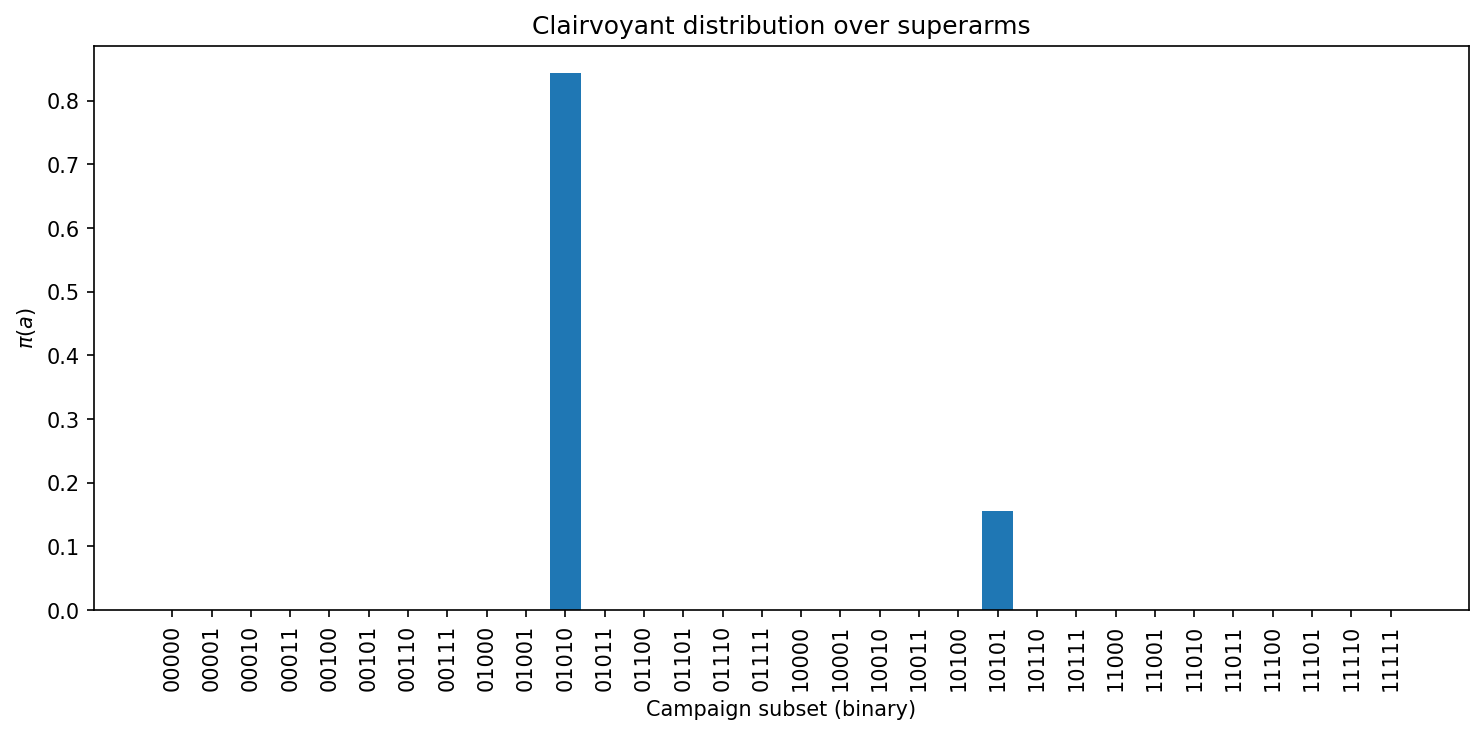
\includegraphics[width=0.8\textwidth]{figures/req2_true_clairvoyant_superarm_distribution.png}\\
    \scriptsize
    A randomized distribution over all the subsets of campaigns optimized by the clairvoyant of Requirement 2. We do not show the conditional distributions over bids within the single campaigns, since they can differ from one subset to another.
\end{frame}

% ============================================================
% Combinatorial-UCB
% ============================================================
\begin{frame}{Combinatorial-UCB: algorithm}
    Implements the UCB-like bidding approach for a combinatorial set of joint actions (i.e., bids on multiple campaigns)

    
    \begin{block}{Core idea}
        \vspace{-0.5cm}
        \[\boxed{\text{UCB estimates} \> + \> \text{conflict-aware campaigns subset optimization} \> + \> \text{budget constraint}}\]
    \end{block}

    \vspace{0.2cm}

    \begin{itemize}
        \item \textbf{Exploration rounds (first $K$ rounds):} randomly-chosen feasible superarms, aiming to explore as many arms as possible
        \begin{itemize}
            \item Some arms might not be chosen $\implies$ no problem, confidence radius gets set to 1 so that they will be explored afterwards
        \end{itemize}
        \item \textbf{Action selection:} we could, as in the single-campaign setting, solve the same LP as the clairvoyant and then sample a bid from the resulting optimal distribution...
    \end{itemize}
\end{frame}

\begin{frame}{Combinatorial-UCB: simpler approach}
    \footnotesize...but it's kinda expensive to do that \emph{every single round}! Instead, we split the clairvoyant LP into two suboptimal (but simpler) Linear Programs:
    \begin{itemize}
        \item First, we solve the single-campaign LP from Requirement 1 with per-round budget $\rho$ to obtain an optimal distribution $\gamma^{(i)}$ over bids for each campaign;
        \item Then, we use the solutions $\gamma^{(i)}$ to form expected utilities/costs for each campaign, and we select a distribution $\gamma_s^\star$ over campaigns subsets through the following LP over all the campaign subsets:
    \end{itemize}

    \vspace{-0.2cm}

    \footnotesize\begin{equation*}
        \begin{aligned}
            \gamma_s^\star = \arg & \max_{\gamma_s \in \mathbb{R}^{2^N}} ~~~ \sum_S \gamma_s(S) \left(\sum_{i \in S} \bar{f}^{(i)}(\gamma^{(i)})\right) \\
            & \begin{aligned} 
                \text{s.t.} ~~~~~~~~~ & \sum_S \gamma_s(S) \left(\sum_{i \in S} \bar{c}^{(i)}(\gamma^{(i)})\right) \le \rho \quad & \text{(budget)} \\
                & \sum_S \gamma_s(S) = 1 & \text{(subset probability)} \\
                & \gamma_s(S) = 0 \quad \forall S \text{ having conflicts} & \text{(conflict)} \\
                & 0 \le \gamma_s(S) \le 1 \quad \forall S \\
            \end{aligned}
        \end{aligned}
    \end{equation*}
\end{frame}

\begin{frame}{True clairvoyant against simplified clairvoyant}
    \begin{alertblock}{}
        We can also use this approach to build a clairvoyant; however, experimental results show that this approach achieves a little less expected utility than the true clairvoyant that we explained earlier
        $\implies$ for this reason, we use this approach only in the Combinatorial-UCB algorithm, but we keep the true clairvoyant for computing the regret
    \end{alertblock}

    \vspace{0.2cm}
    
    \centering
    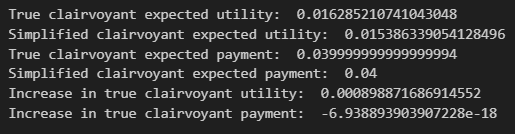
\includegraphics[width=0.6\textwidth]{figures/req2_true_clairvoyant_against_simplified_clairvoyant.PNG}
\end{frame}

% ============================================================
% Splitting the problem
% ============================================================
\begin{frame}{Explosion of LP variables}
    \centering
    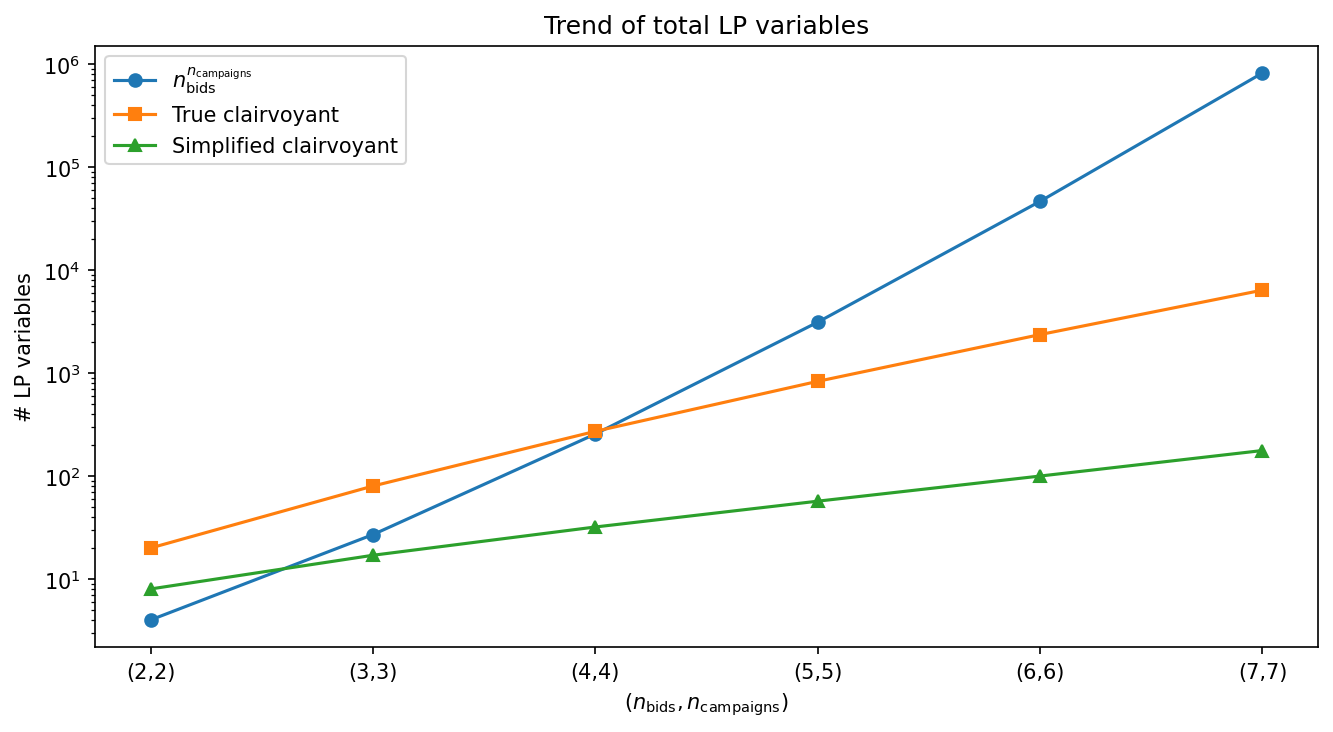
\includegraphics[width=0.7\textwidth]{figures/req2_lp_variables_trend.png}\\
    \scriptsize
    Comparison of the variables in the three possibilities for the LP: \textcolor{blue}{full joint distribution} (LP not analyzed in these slides), \textcolor{orange}{distribution from true clairvoyant}, \textcolor{green}{distribution from simplified clairvoyant}. Note that the y-axis is logarithmic.
\end{frame}

% ============================================================
% Results
% ============================================================
\begin{frame}{Results: Combinatorial-UCB using true LP}
    \begin{columns}[T]
        \begin{column}{0.6\textwidth}
            \centering
            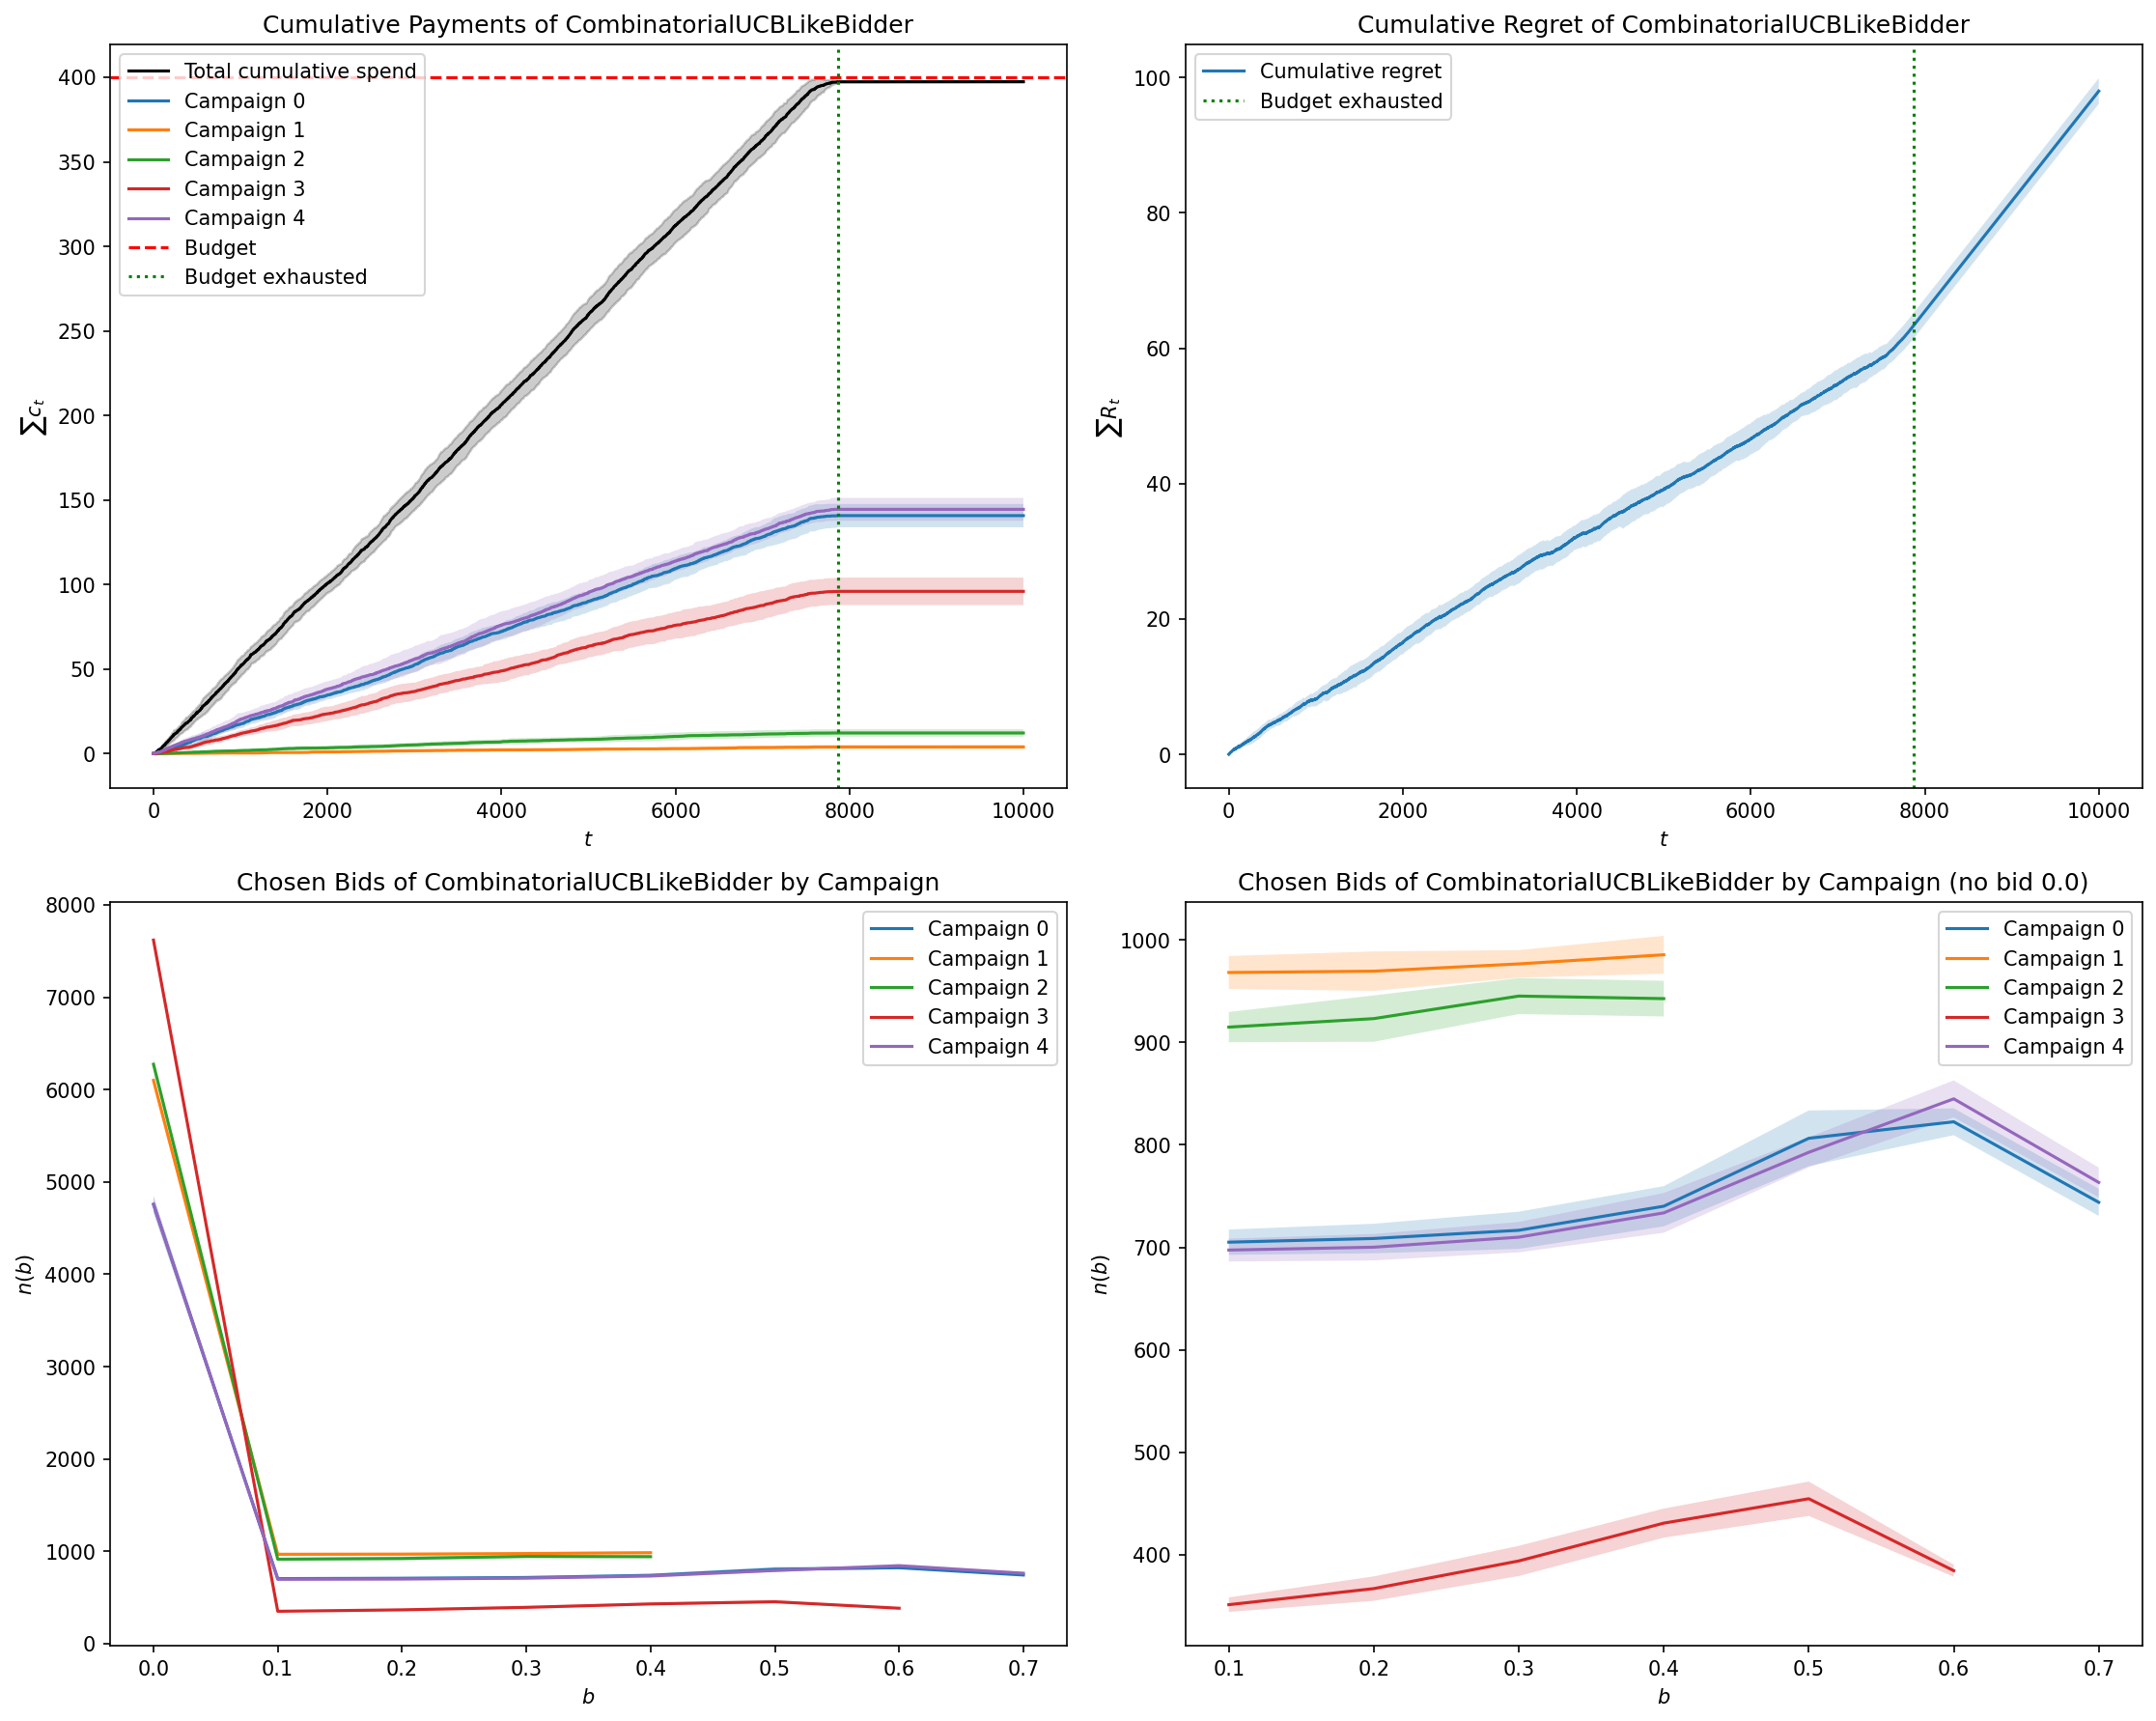
\includegraphics[width=0.9\textwidth]{figures/req2_true_true_experiment_results.png}\\
        \end{column}
        \begin{column}{0.3\textwidth}
             \begin{itemize}
                \item $10000$ (!) rounds are not enough to get evident sublinear regret and a clear separation among bids, although a hint of a peak among the bids of some campaigns can be seen
                \item Randomizing among subsets of campaigns leads to each campaign not being played sometimes
            \end{itemize}
        \end{column}\hfill
    \end{columns}
\end{frame}

\begin{frame}{Results: Combinatorial-UCB using simplified LP}
    \begin{columns}[T]
        \begin{column}{0.6\textwidth}
            \centering
            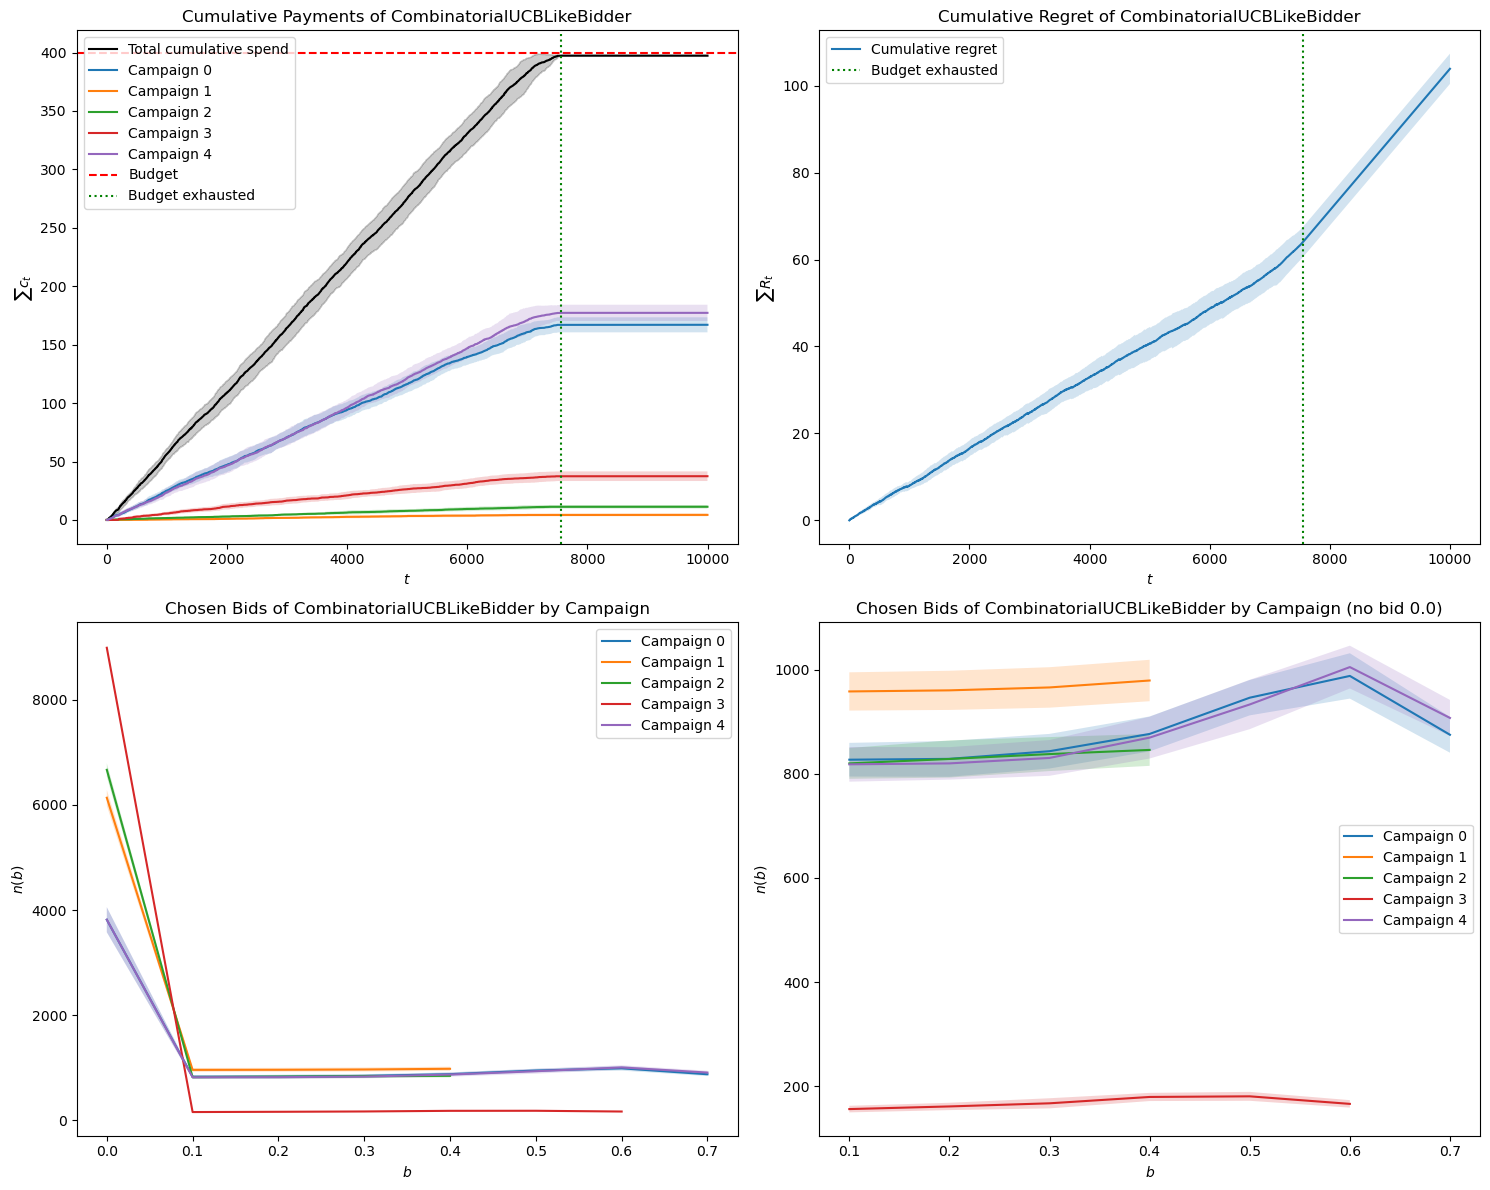
\includegraphics[width=0.9\textwidth]{figures/req2_simplified_true_experiment_results.png}\\
        \end{column}
        \begin{column}{0.3\textwidth}
             \begin{itemize}
                \item The regret is similar to that achieved using the true LP
                \item The separation between bids played is even less clear
            \end{itemize}
        \end{column}\hfill
    \end{columns}
\end{frame}

\begin{frame}{Results: comparison of the regrets of the two variants}
    \centering
    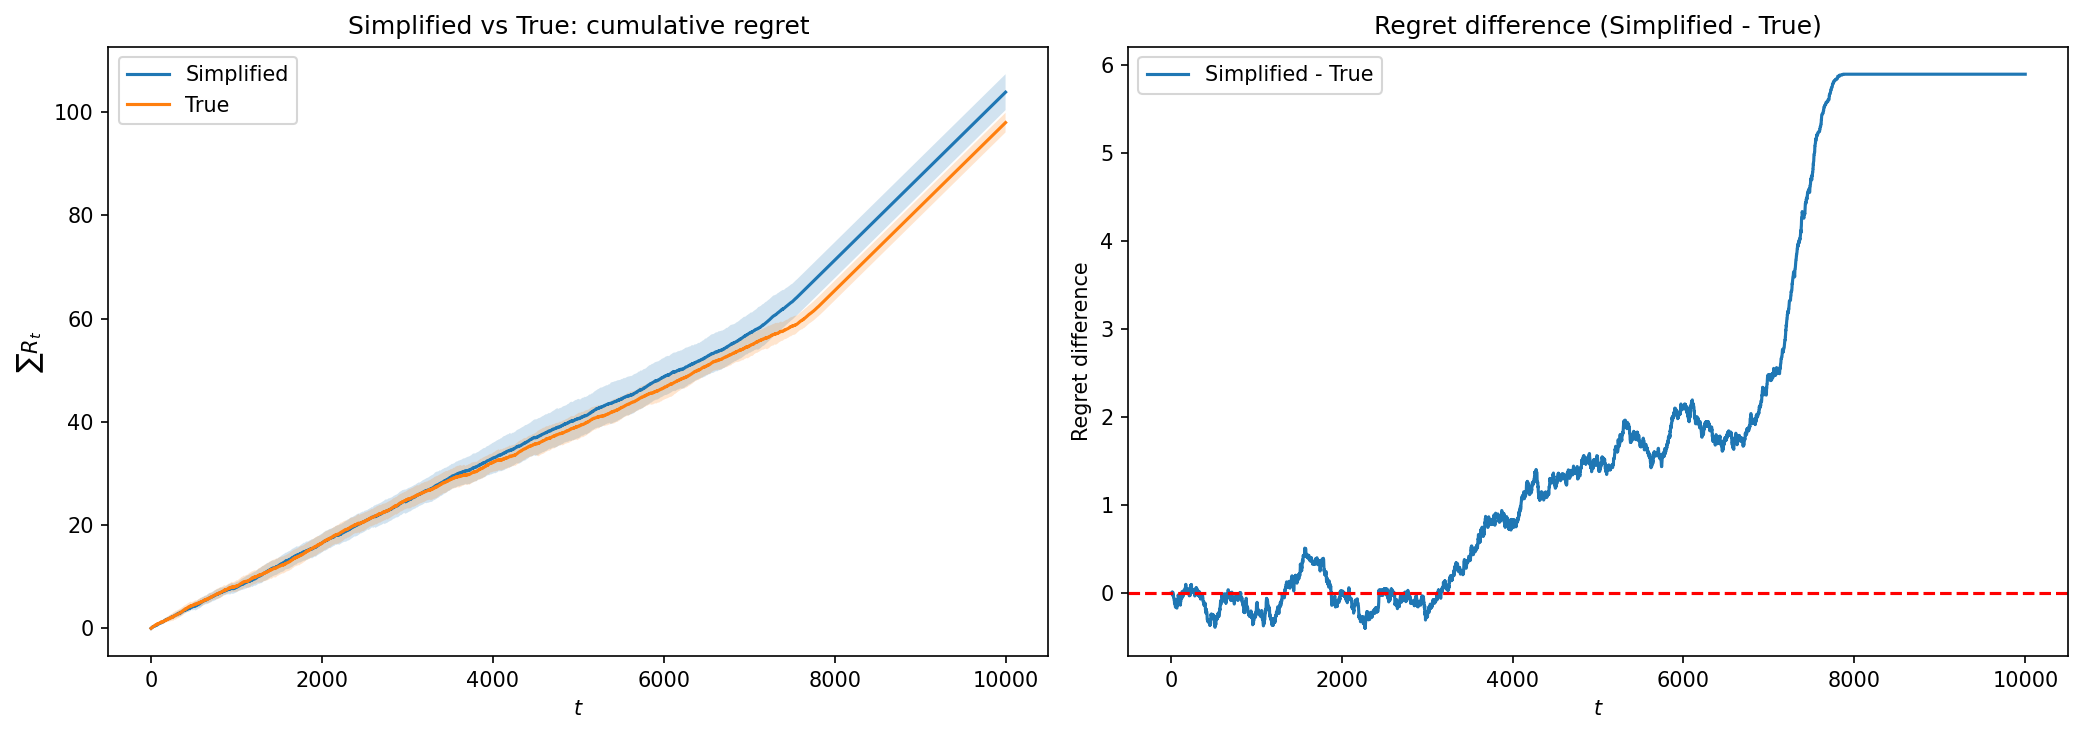
\includegraphics[width=\textwidth]{figures/req2_simplified_vs_true_regret.png}\\
    \scriptsize
    The Combinatorial-UCB bidder that uses the true LP achieves a little less regret than the bidder using the simplified LP (but also takes three times as much time to execute $\implies$ probably not worth it!).
\end{frame}


\section{Requirement 3: highly non-stationary multiple-campaigns environment}

% ============================================================
% Overview
% ============================================================
\begin{frame}{Highly non-stationary multiple-campaigns environment}
    \begin{itemize}
        \item Sequence of highest competing bids $(m_t^{(i)})_t$ sampled from a distribution that \emph{changes quickly and continuously over time}
        \item Different patterns per campaign but possibly \emph{correlated} through market regimes (e.g., holidays, Black Friday)
        \item UCB-style methods break: confidence radius assumes stationarity
        \item Algorithm to be studied: \textbf{primal-dual} with budget, assuming full feedback
        \begin{itemize}
            \item Full-feedback: highest competing bid $m_t^{(i)}$ is observed, providing information about all arms regardless of which one we bid on
            
            $\implies$ a regret minimizer for the adversarial expert problem (\textbf{Hedge}) is appropriate!
        \end{itemize}
    \end{itemize}
\end{frame}

% ============================================================
% Distribution model
% ============================================================
\begin{frame}{Distribution model: adversarial-style sinusoids}
    \begin{columns}[T]
        \lfill\begin{column}{0.4\textwidth}
            \small\textbf{Modeling choice:}
            \begin{itemize}
                \item Each competitor's bid at round $t$ is drawn from $\mathrm{Unif}(0, u^{(i)}_t)$ where
                \begin{equation*}
                    \begin{aligned}
                        u^{(i)}_t &= low^{(i)} + \\ 
                        & (high^{(i)} - low^{(i)})\bigl(1 - |\sin(5t/T)|\bigr)
                    \end{aligned}
                \end{equation*}
            \end{itemize}
        \end{column}
        \begin{column}{0.45\textwidth}
            \centering
            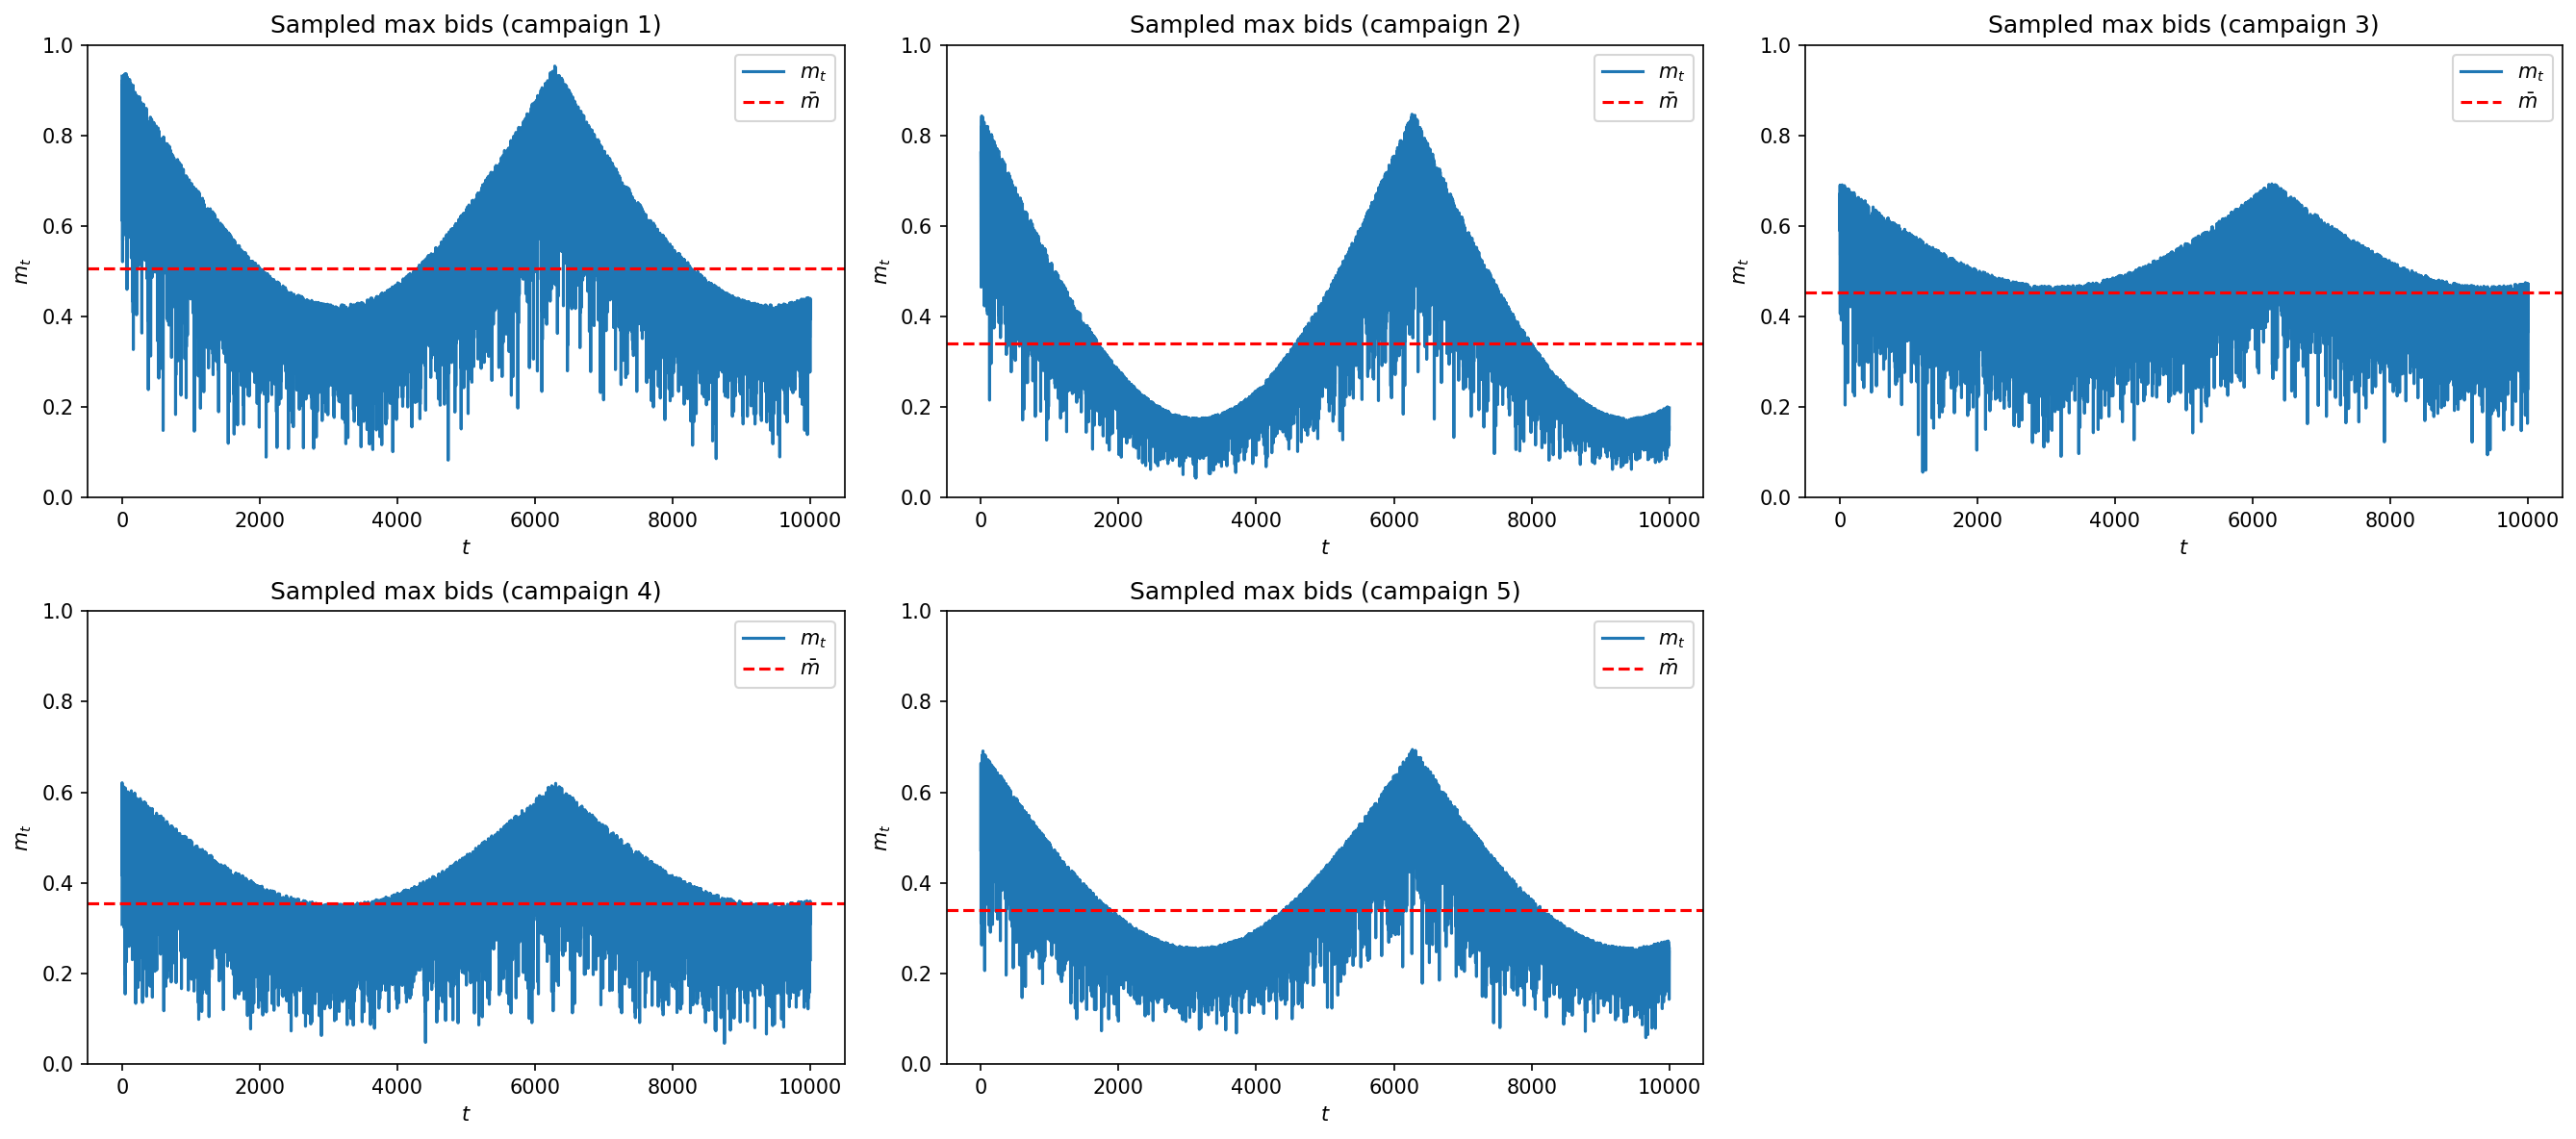
\includegraphics[width=\textwidth]{figures/req3_max_bids_ts.png}
        \end{column}
    \end{columns} 

    \vspace{0.1cm}

    \small\begin{itemize}
        \item Same frequency across campaigns: models price changes due to the \emph{shared market conditions}, like sales (Black Friday), holidays (Christmas), \ldots during which showing ads is more valuable and competitors are likely to bid more
        \item $high$ and $low$ represent the range of the oscillations
        \item Max of uniforms is Beta-distributed \emph{within each round}, but the parameters change continuously, so the Beta distribution is actually rescaled
    \end{itemize}
\end{frame}

% ============================================================
% Clairvoyant LP - highly non-stationary
% ============================================================
\begin{frame}{Clairvoyant}
    \begin{itemize}
        \item We want to use a similar LP to that of the clairvoyant for Requirement 2
        \item The previous clairvoyants used the true win probabilities $\mathbb{P}\left[ m \le b \right]$ from the known underlying stationary distribution 
        \item But: now, the distribution of the highest competing bids keeps changing quickly throughout the rounds $\implies$ no fixed win probabilities!
    \end{itemize}

Instead, use the estimates $\hat{\mathbb{P}}\left[ m \le b \right]$ of the empirical win probabilities (computed in hindsight)!
        
    \begin{block}{Assumption} 
        The clairvoyant knows the empirical win probability $\hat{\mathbb{P}}\left[ m \le b \right]$ a posteriori of each bid $b$ (like in the exercise session).
    \end{block}
\end{frame}

\begin{frame}{Clairvoyant: from Requirement 2 to Requirement 3}
    \vspace{-0.4cm}
    \footnotesize\begin{equation*}
        \begin{aligned}
            \gamma_s^\star, [\gamma_i]^\star = \arg & \max_{\gamma_s \in \mathbb{R}^{2^N}, [\gamma_{S, i}] \in \mathbb{R}^{NK}} ~~~ \sum_S \sum_{i \in S} \sum_b \gamma_{S, i}(b)\, \textcolor{red}{\bar{f}^{(i)}(b)} \\
            & \begin{aligned} 
                \text{s.t.} ~~~~~~~~~~~~~~~~~~ & \sum_S \sum_{i \in S} \sum_b \gamma_{S, i}(b)\, \textcolor{red}{\bar{c}^{(i)}(b)} \le \rho \quad & \text{(budget)} \\
                & \sum_S \gamma_s(S) = 1 & \text{(subset probability)} \\
                & \sum_b \gamma_{S, i}(b) = \gamma_S(S) \quad \forall S, i & \text{(marginalization)} \\
                & \gamma_{S, i}(0) = 0 \quad \forall S,\, \forall i \in S & \text{(campaign in subset)} \\
                &\gamma_{S, i}(0) = 1 \quad \forall S,\, \forall i \notin S & \text{(campaign not in subset)} \\
                & \gamma_s(S) = 0 \quad \forall S \text{ having conflicts} & \text{(conflict)} \\
                & 0 \le \gamma_s(S) \le 1 \quad \forall S \\
                & 0 \le \gamma_{S, i}(b) \le 1 \quad \forall b 
            \end{aligned}
        \end{aligned}
    \end{equation*}

    The win probabilities affect the LP from within $\textcolor{red}{\bar{f}^{(i)}(b)} = (v - b)\, \mathbb{P}_{m \sim \mathcal{D}_m}\left[ b \ge m \right]$ (and $\textcolor{red}{\bar{c}^{(i)}(b)}$): simply replace $\mathbb{P}_{m \sim \mathcal{D}_m}\left[ b \ge m \right]$ with $\hat{\mathbb{P}}_{m \sim \mathcal{D}_m}\left[ b \ge m \right]$!
\end{frame}

\begin{frame}{Clairvoyant: optimal $\gamma$ under highly non-stationarity}
    \centering
    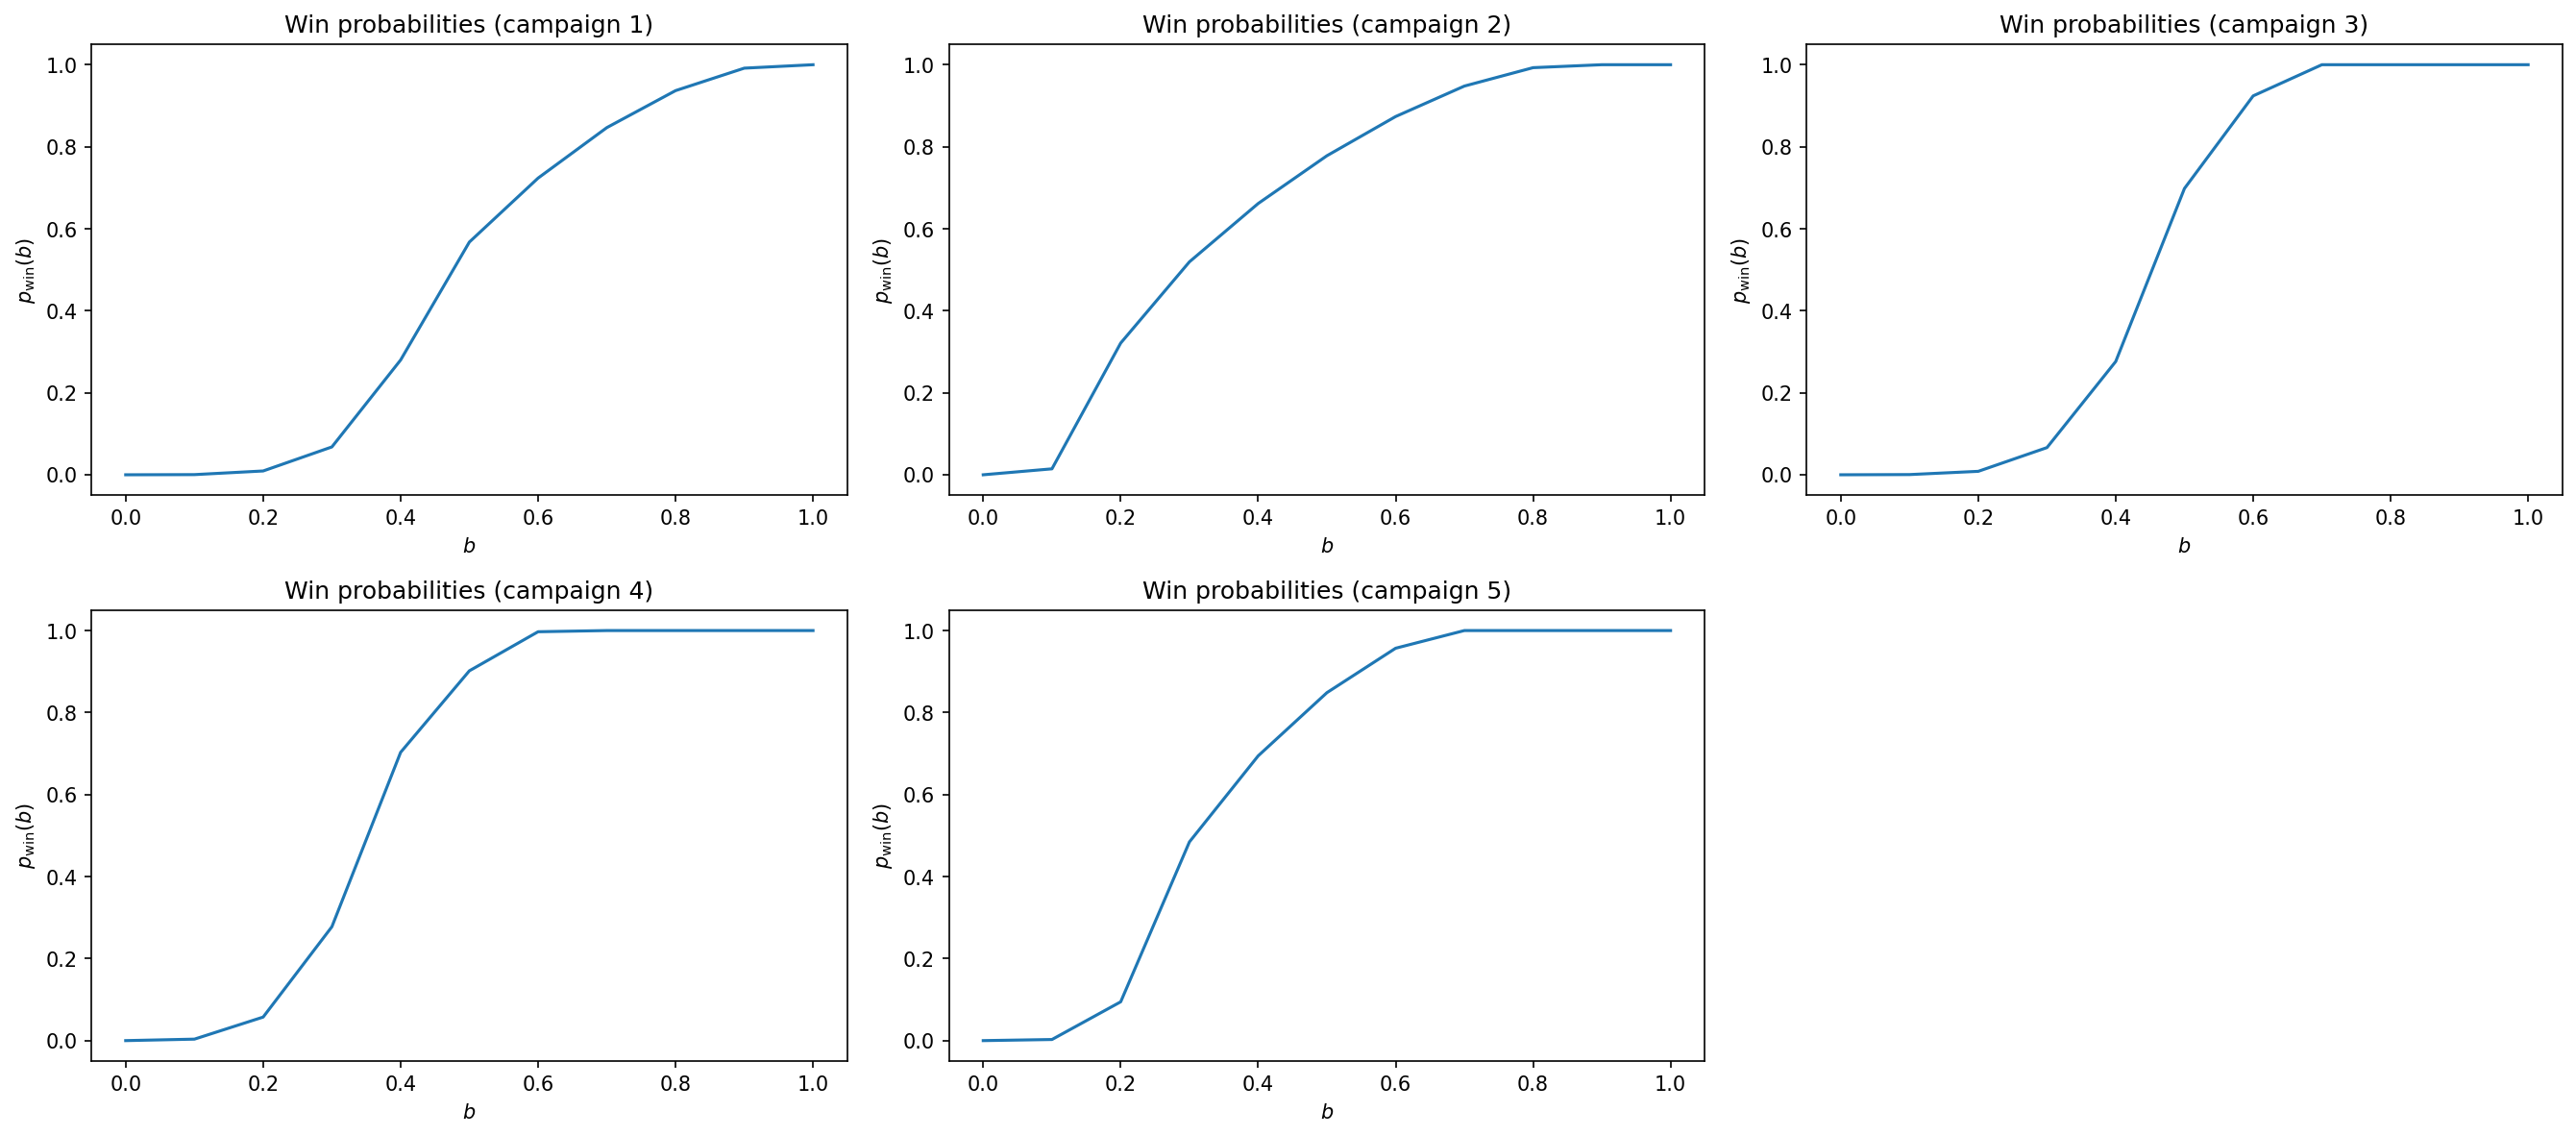
\includegraphics[width=0.5\textwidth]{figures/req3_win_probabilities.png}\hfill
    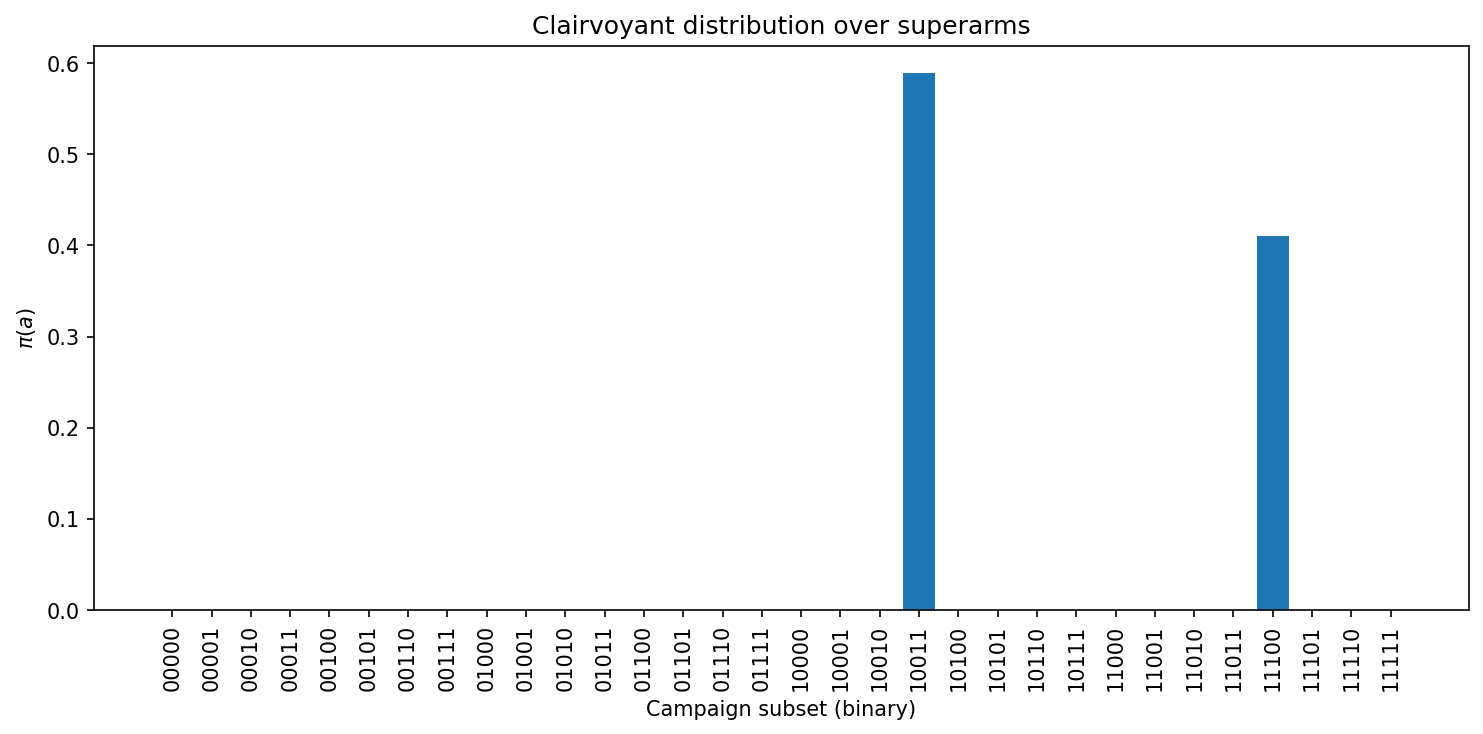
\includegraphics[width=0.48\textwidth]{figures/req3_clairvoyant_superarm.png}\\
    \scriptsize
    \textbf{Left:} empirical $\hat{\mathbb{P}}\left[b \ge m_t\right]$, estimated a posteriori over all rounds.\\
    \textbf{Right:} optimal strategy $\gamma^\star$ of the clairvoyant, which still randomizes over multiple campaigns subsets.
\end{frame}

% ============================================================
% Primal-Dual bidder
% ============================================================
\begin{frame}{Primal-dual bidder: optimization problem}
    \begin{block}{Remember:}
        $\gamma$ is the distribution over joint actions, induced in our case by the two-step sampling procedure
    \end{block}

    The optimization problem that we are solving is 
    \[\gamma^\star = \arg \max_{\gamma \in \Delta_\mathcal{B}} \bar{f}(\gamma) \qquad \text{s.t.  } \bar{c}(\gamma) \le \rho\]

    The probability simplex constraint is already enforced by the choice of Hedge as regret minimizer: the budget constraint is instead incorporated through the expected Lagrangian
    \[\bar{\mathcal{L}}(\gamma, \lambda) = \underbrace{\bar{f}(\gamma)}_{\text{expected utility}} - \lambda(\underbrace{\bar{c}(\gamma)}_{\text{expected payment}} - \rho)\]
    \vspace{0.2cm}
    where $\bar{f}(\gamma) = \sum_{i=1}^N \mathbb{E}_{\mathbf{b} \sim \gamma}\left[ \mathbb{E}_{(m^{(1)}, \cdots, m^{(N)}) \sim \mathcal{D_\mathbf{m}}}\left[ f^{(i)}(b_i, m_i) \right] \right]$ (and same for $\bar{c}(\gamma)$)
\end{frame}

\begin{frame}{Primal-dual bidder: structure}
    \begin{itemize}
        \item \textbf{Dual step (stochastic gradient ascent on $\lambda$):}
        \[\boxed{\lambda_{t+1} = \Pi_{[0,1/\rho]} \left(\lambda_t - \eta_d\,(\rho - c_t) \right)}\]

        in which $c_t$ is estimating $\bar{c}(\gamma)$ in the expected Lagrangian
    \end{itemize}
\end{frame}

\begin{frame}{Primal-dual bidder: structure}
    \begin{itemize}
        \item \textbf{Primal step (multiplicative Hedge updates on $\gamma$):} $N + 1$ separate Hedge instances on
        \begin{itemize}
            \item $N$ per-campaign bid distributions $\gamma_i$ over $\mathcal{B}\, \backslash\, \{0.0\} \rightarrow$ Hedge updates: \[w_{t+1}^{(i)}(b) = w_t^{(i)}(b)\, e^{-\eta_p \ell_t^{(i)}(b)} \quad \forall b \in \mathcal{B}\]
            \item campaigns-subsets distribution $\gamma_s$  $\rightarrow$ Hedge updates: \[w_{t+1}(S) = w_t(S)\, e^{-\eta_p \mathcal{L}_t(S)} \quad \forall S \in \mathcal{\mathcal{P}(N)}\]
        \end{itemize}
    \end{itemize}

    \begin{block}{}
        Same decomposition as the Combinatorial-UCB bidder in Requirement 2!
    \end{block}
    
    \begin{block}{}
        Conflicts are masked by initializing to $0$ the weights corresponding to invalid superarms: Hedge's multiplicative updates won't be able to change these weights
    \end{block}
\end{frame}

\begin{frame}{Primal-dual bidder: structure}
    \begin{itemize}
        \item \textbf{Primal step (multiplicative Hedge updates on $\gamma$):} 
        \[w_{t+1}^{(i)}(b) = w_t^{(i)}(b)\, e^{-\eta_p \textcolor{red}{\ell_t^{(i)}(b)}} \quad \forall b \in \mathcal{B}\]
        \[w_{t+1}(S) = w_t(S)\, e^{-\eta_p \textcolor{red}{\mathcal{L}_t(S)}} \quad \forall S \in \mathcal{\mathcal{P}(N)}\]

        \begin{block}{}
            We actually use two kinds of Lagrangians for the primal step: one "global" Lagrangian $\mathcal{L}_t$ (like the dual one) for Hedge over the campaigns subsets, and single-campaign Lagrangians $\ell_t$ for the Hedge instances over the single campaigns
        \end{block}
    \end{itemize}
\end{frame}

\begin{frame}{Primal-dual bidder: Lagrangians}
    At round $t$, we observe the highest competing bid $m_t^{(i)}$ for all bids in all campaigns:
    \begin{itemize}
        \item $f_t^{(i)}(b_i) = (v_i - b_i)\,\mathds{1}\left[ b_i \geq m_t^{(i)} \right]$ is the utility obtained from campaign $i$ if playing bid $b_i$
        \item $c_t^{(i)}(b_i) = b_i\,\mathds{1}\left[ b_i \geq m_t^{(i)} \right]$ is the payment for campaign $i$ if playing bid $b_i$
    \end{itemize}

    \vspace{1cm}

    The overall expected utility and payment for any subset $S$ of campaigns are
    \[f_t(S) = \sum_{i \in S} \mathbb{E}_{\mathbf{b} \sim \gamma_{i|S}}\left[ f_t^{(i)}(b_i) \right] = \sum_{i \in S} f_t^{(i)}(\gamma_{i|S}), \quad c_t(S) = \sum_{i \in S} \mathbb{E}_{\mathbf{b} \sim \gamma_{i|S}}\left[ c_t^{(i)}(b_i) \right] = \sum_{i \in S} c_t^{(i)}(\gamma_{i|S}).\]
\end{frame}

\begin{frame}{Primal-dual bidder: Lagrangians}
    With the budget constraint $c_t \leq \rho$, the global per-round Lagrangian is
    \[\boxed{\mathcal{L}_t(S, \lambda_t) = f_t(S) - \lambda_t(c_t(S) - \rho)}\]

    \vspace{-0.2cm}

    \begin{alertblock}{Key point}
        The term $\lambda_t\rho$ appears \textbf{once}, regardless of
        how many cammpaigns ($|S|$) are in subset $S$
    \end{alertblock}

    \vspace{0.2cm}

    The single-campaign Lagrangians, instead, only use $f_t^{(i)}(b_i)$ and $c_t^{(i)}(b_i)$ of one campaign:
    \[\boxed{\ell_t^{(i)}(b_i, \lambda_t) = f_t^{(i)}(b_i) - \lambda_t (c_t^{(i)}(b_i) - \rho)}\]
\end{frame}

% ============================================================
% Results: dual variable
% ============================================================
\begin{frame}{Results: dual variable $\lambda_t$ and per-round expense}
    \begin{columns}[T]
        \begin{column}{0.55\textwidth}
            \hfill
            \centering
            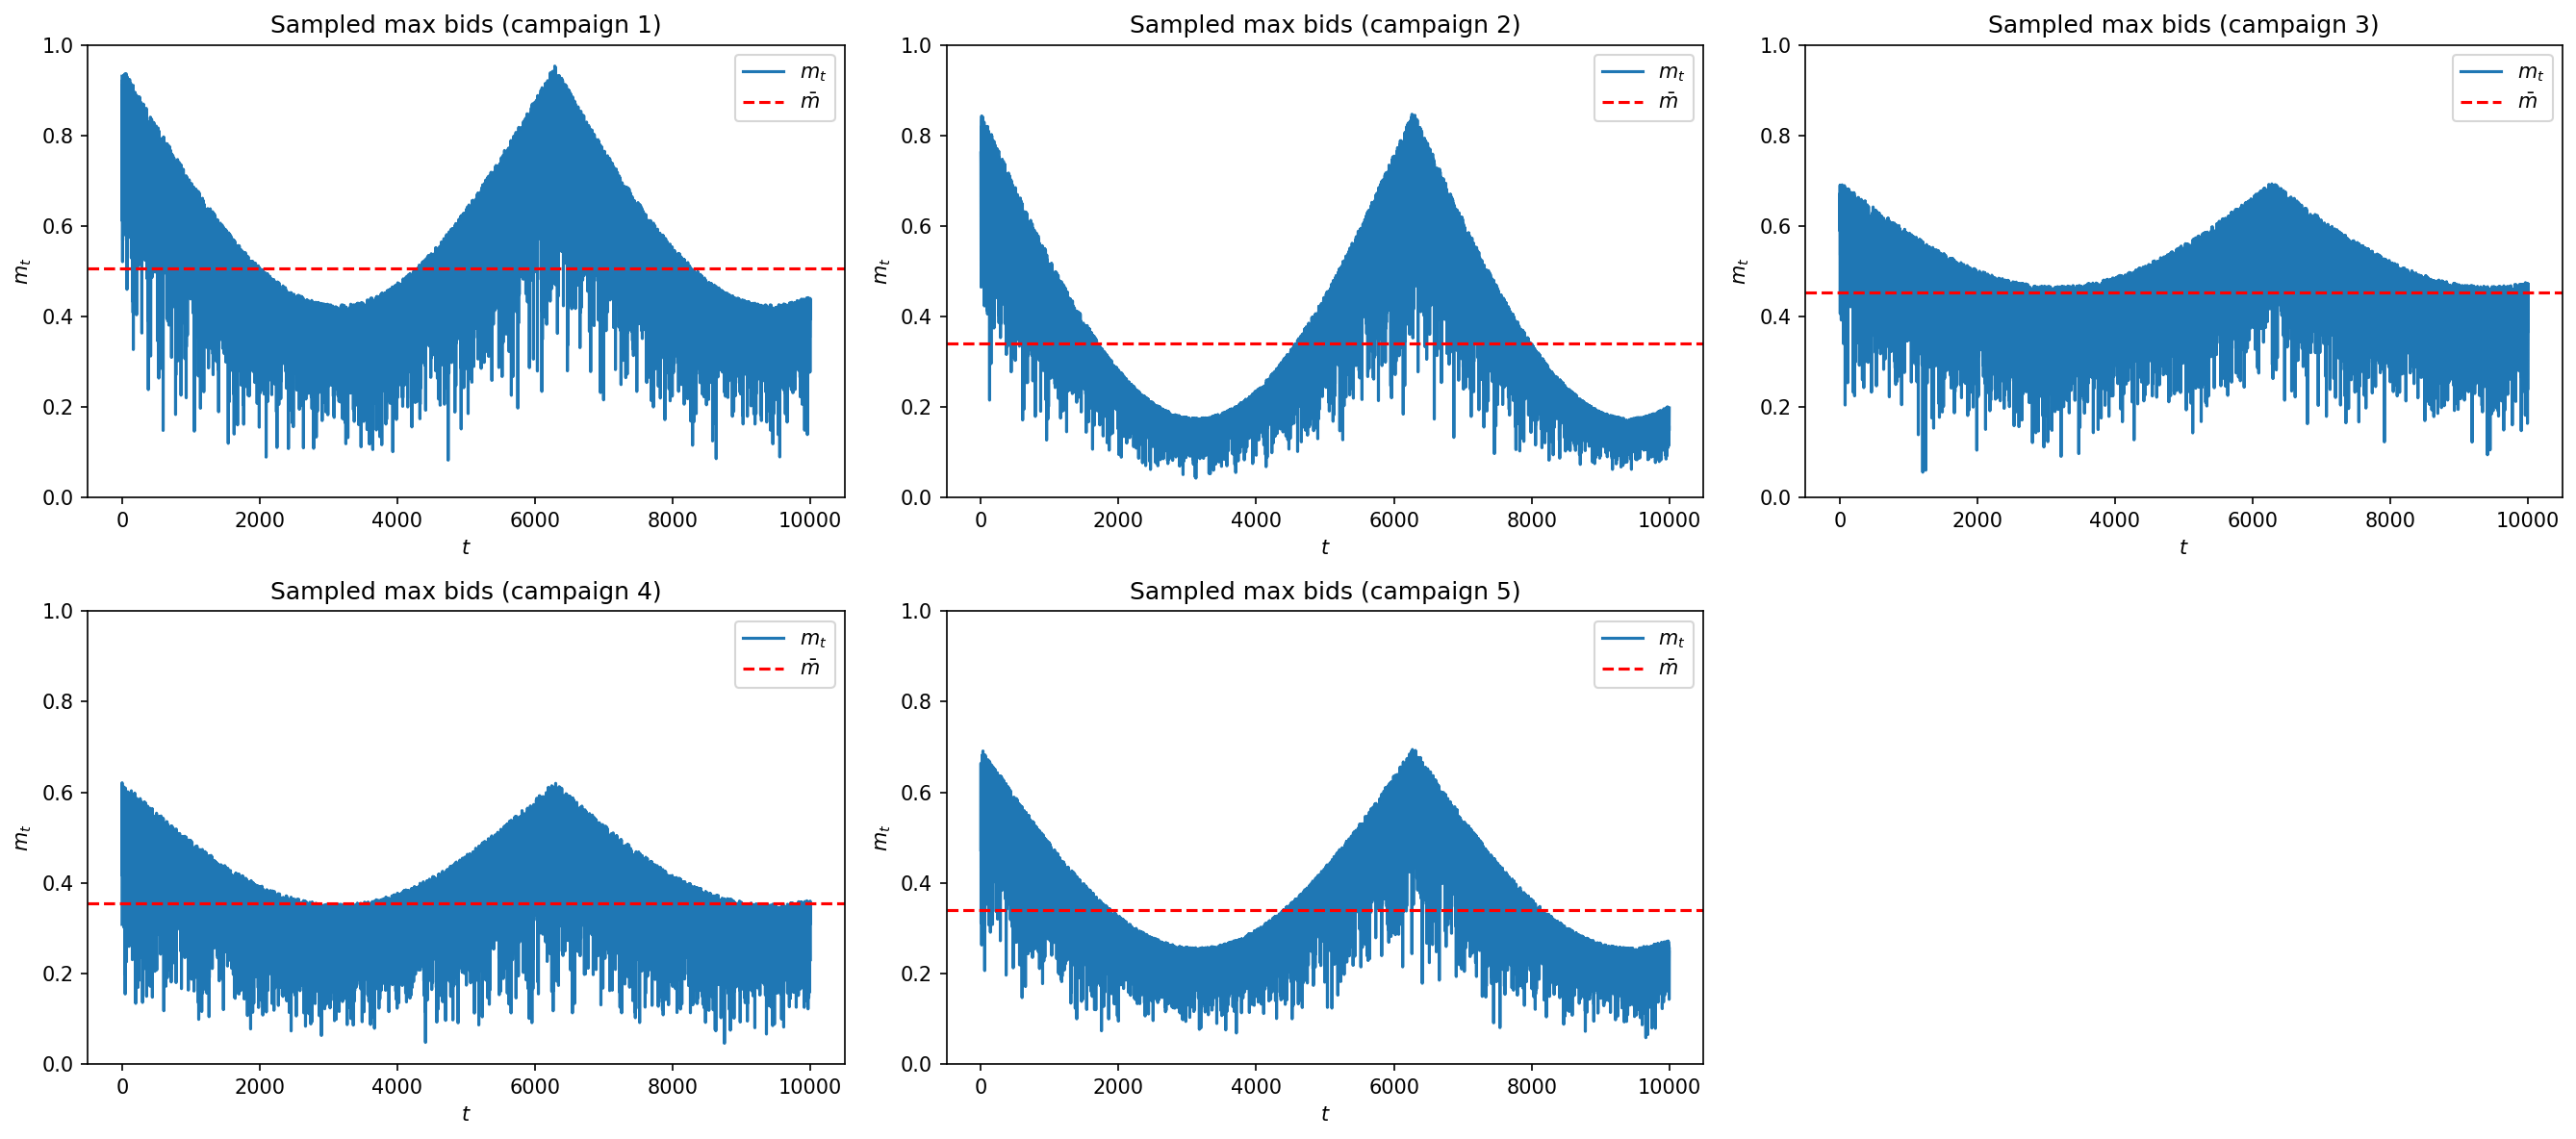
\includegraphics[width=0.95\textwidth]{figures/req3_max_bids_ts.png}\\
            \scriptsize
            $\lambda_t$ drifts upward or downward (\textbf{right: top plot}) respectively when the bidder spends less or more than $\rho$ (\textbf{right: bottom plot}). 
            \begin{itemize}
                \item During the peaks in the \textbf{left plot}, $\lambda_t$ decreases, counteracting the need of spending more due to the overall higher competing bids;
                \item during the valleys, lambda grows, because the current auctions being less expensive means that we could try to win them more often.
            \end{itemize} 
        \end{column}
        \begin{column}{0.35\textwidth}
            \centering
            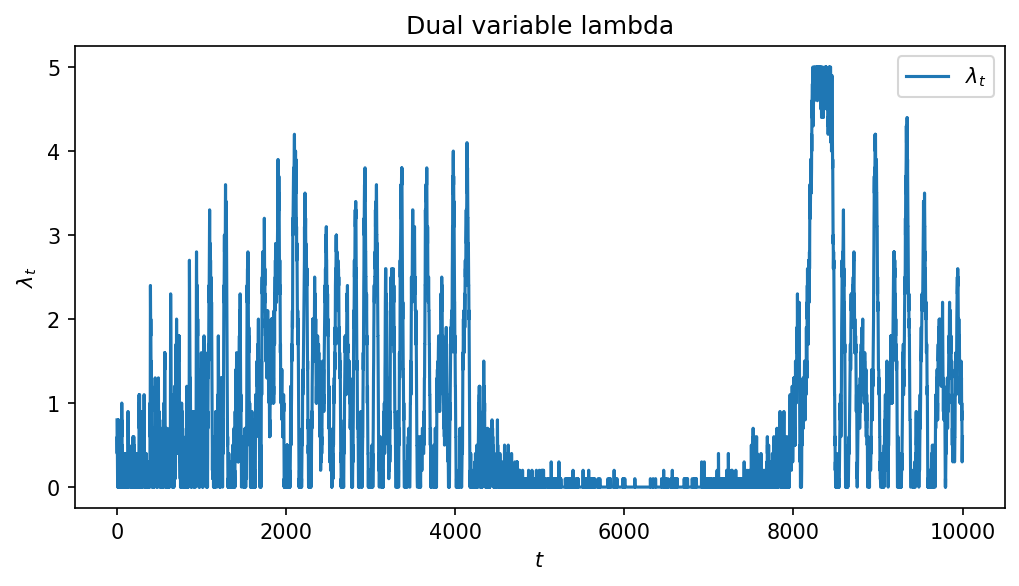
\includegraphics[width=1.1\textwidth]{figures/req3_dual_lambda.png}\\
            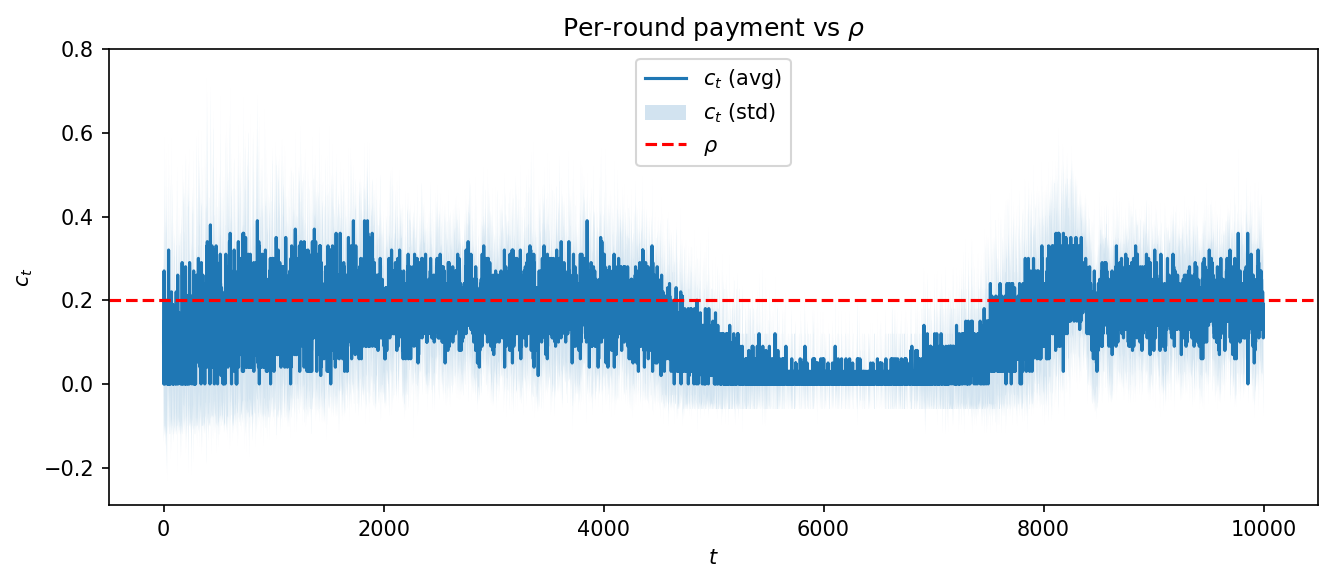
\includegraphics[width=1.1\textwidth]{figures/req3_per_round_payment_vs_rho.png}\\
        \end{column}\hfill
    \end{columns}
     
\end{frame}

% ============================================================
% Results: cumulative regret & payments
% ============================================================
\begin{frame}{Results: primal-dual}
    \begin{columns}[T]
        \begin{column}{0.6\textwidth}
            \centering
            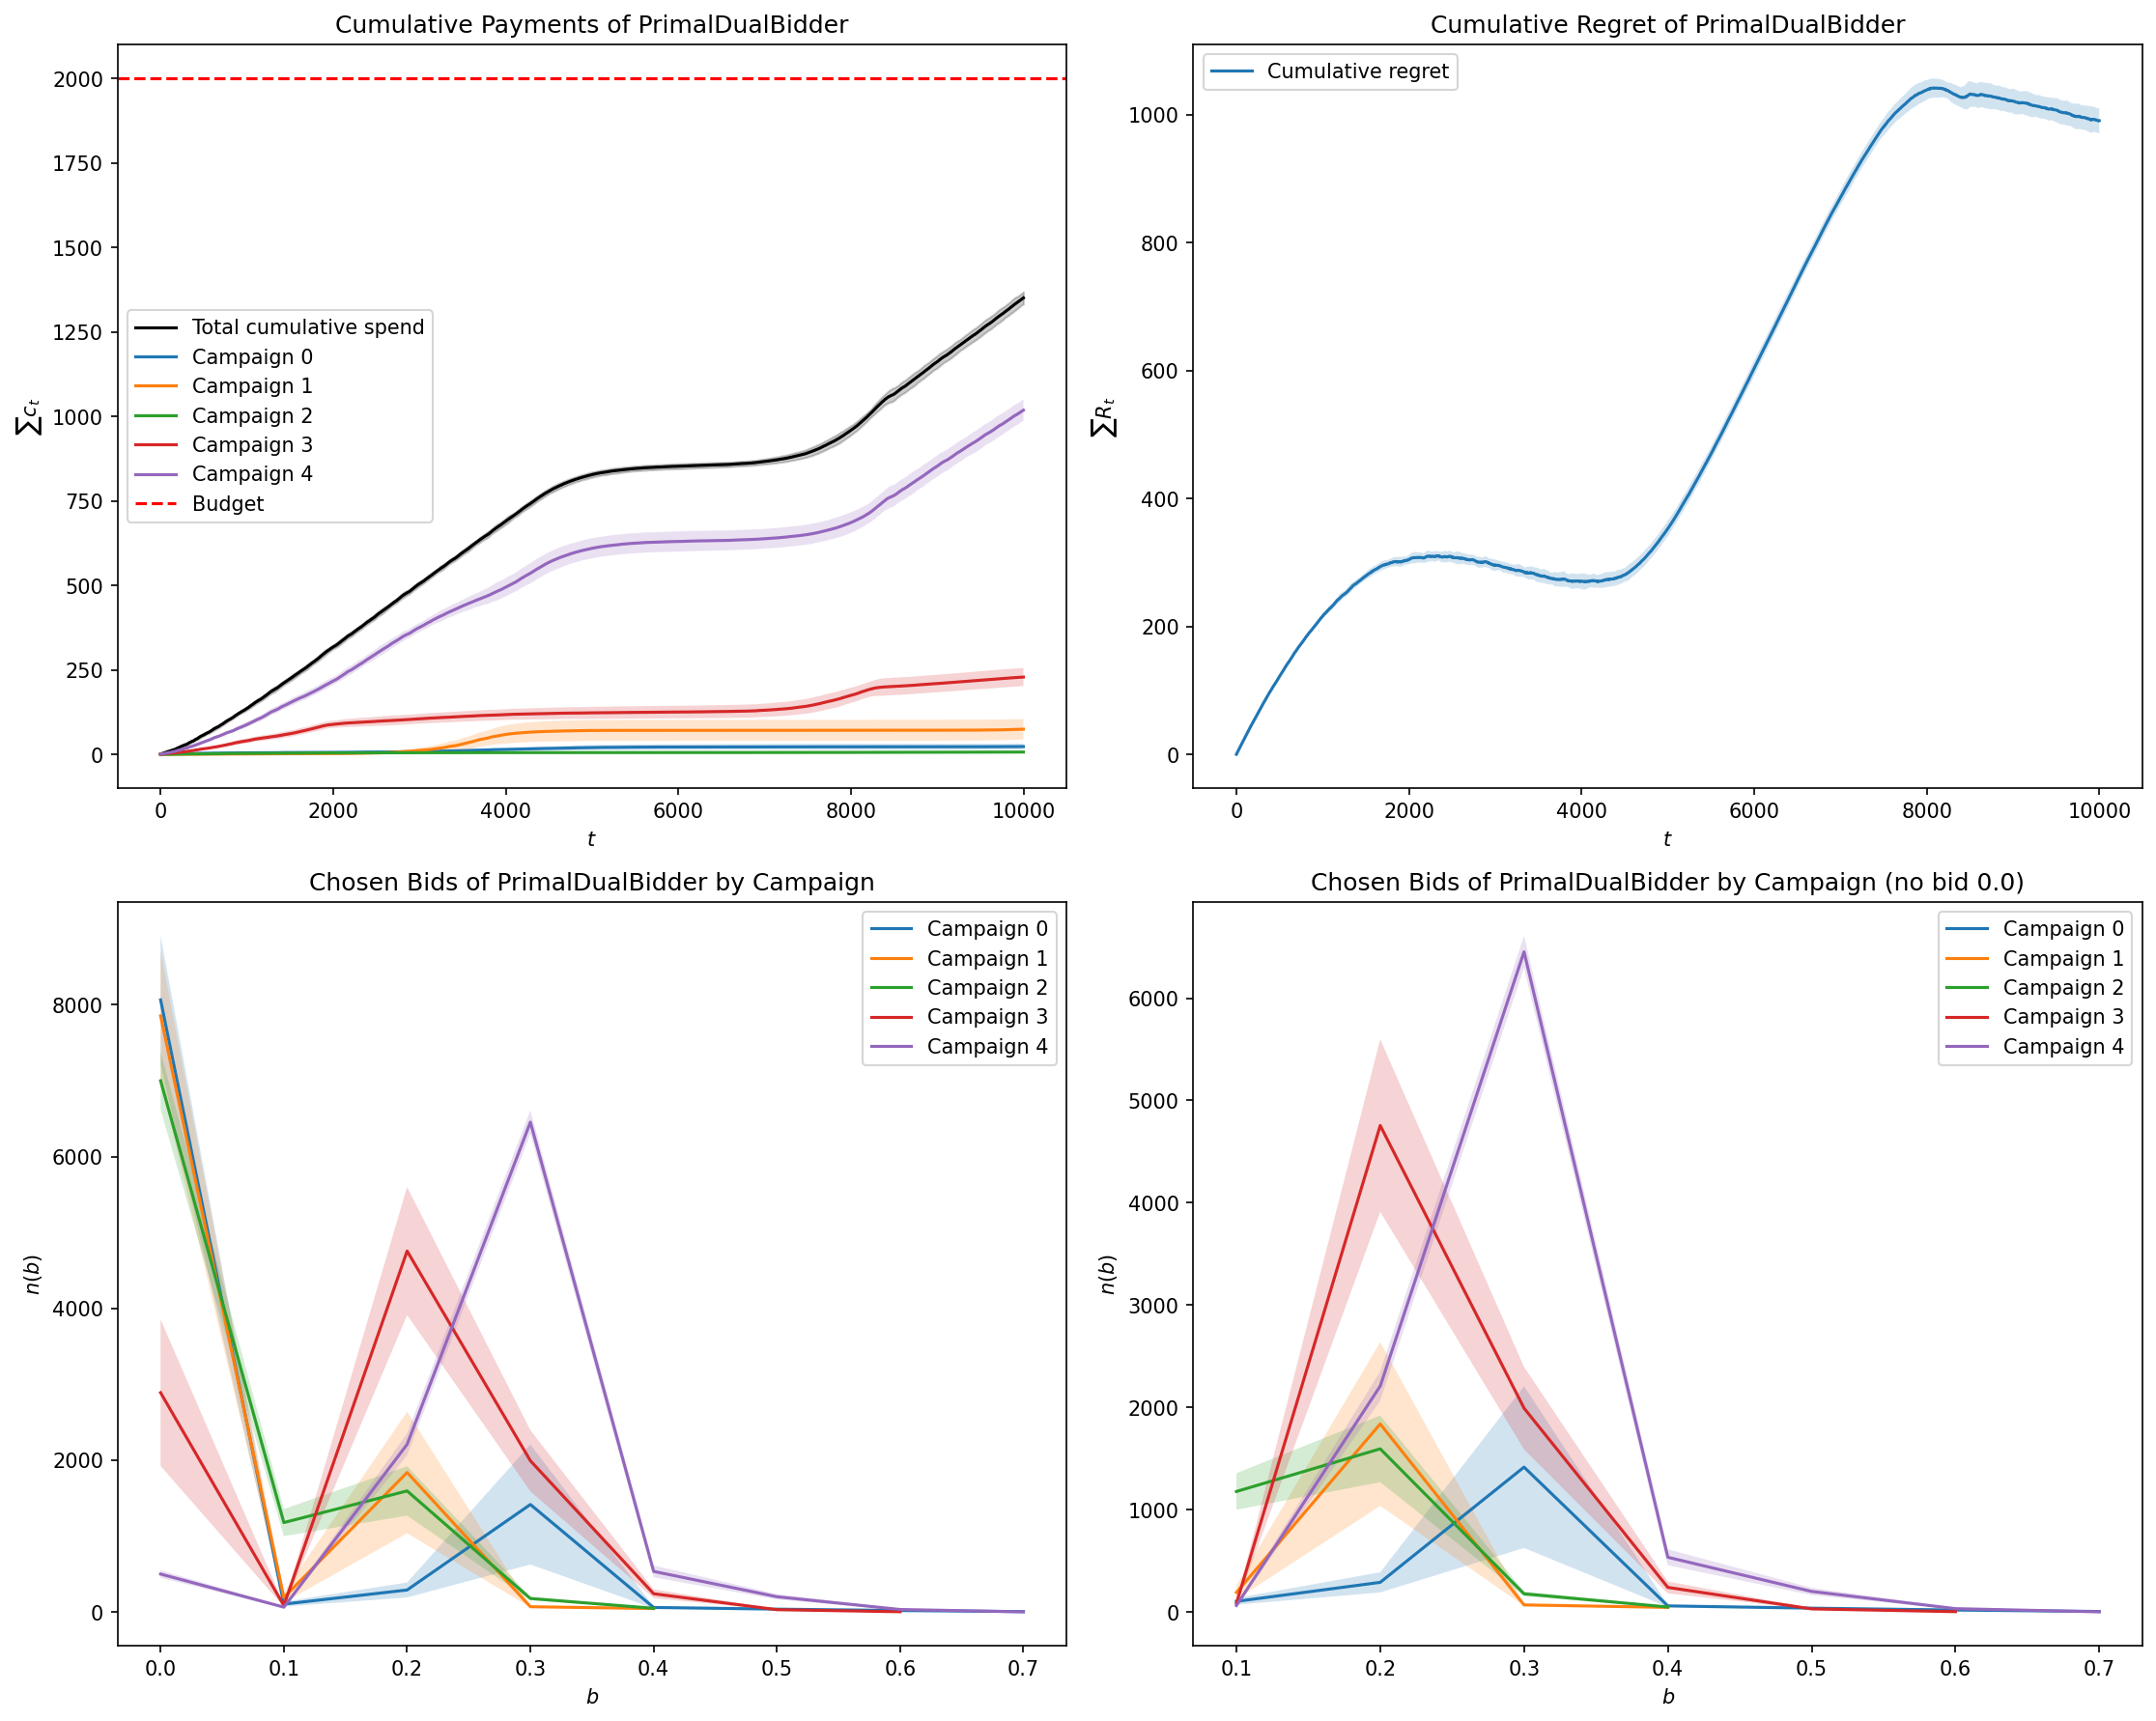
\includegraphics[width=0.9\textwidth]{figures/req3_primal_dual_experiment_results.png}\\
        \end{column}
        \begin{column}{0.4\textwidth}
             \footnotesize\begin{itemize}
                \item The primal-dual bidder is very conservative and spends much less than the budget
                \item This happens whatever the budget is: this bidder never depletes all the budget (observed while making attempts, but not in the notebook)
                \item Regret is sublinear, but clearly follows the trend in the highest competing bids
                \item Bids are (surprisingly) clearly separated: the primal-dual bidder likely acts on the pacing of the bids (how often), not on the value of the bid itself
            \end{itemize}
        \end{column}\hfill
    \end{columns}
\end{frame}

\section{Requirement 4: slightly non-stationary multiple-campaigns environment}

% ============================================================
% Overview
% ============================================================
\begin{frame}{Slightly non-stationary multiple-campaigns environment}
    \begin{itemize}
        \item Rounds partitioned in \emph{stationary intervals} (phases), each with its own joint distribution of highest competing bids $m_p^{(i)}$
        \item Algorithms to be compared:
        \begin{itemize}
            \item \textbf{Combinatorial-UCB with sliding window}
            \item \textbf{Combinatorial-UCB with CUSUM change detection}
            \item \textbf{Primal-dual} (same as Req 3, no change awareness)
        \end{itemize}
    \end{itemize}
\end{frame}

% ============================================================
% Distribution model
% ============================================================
\begin{frame}{Distribution model: piecewise-stationary phases}
    \centering
    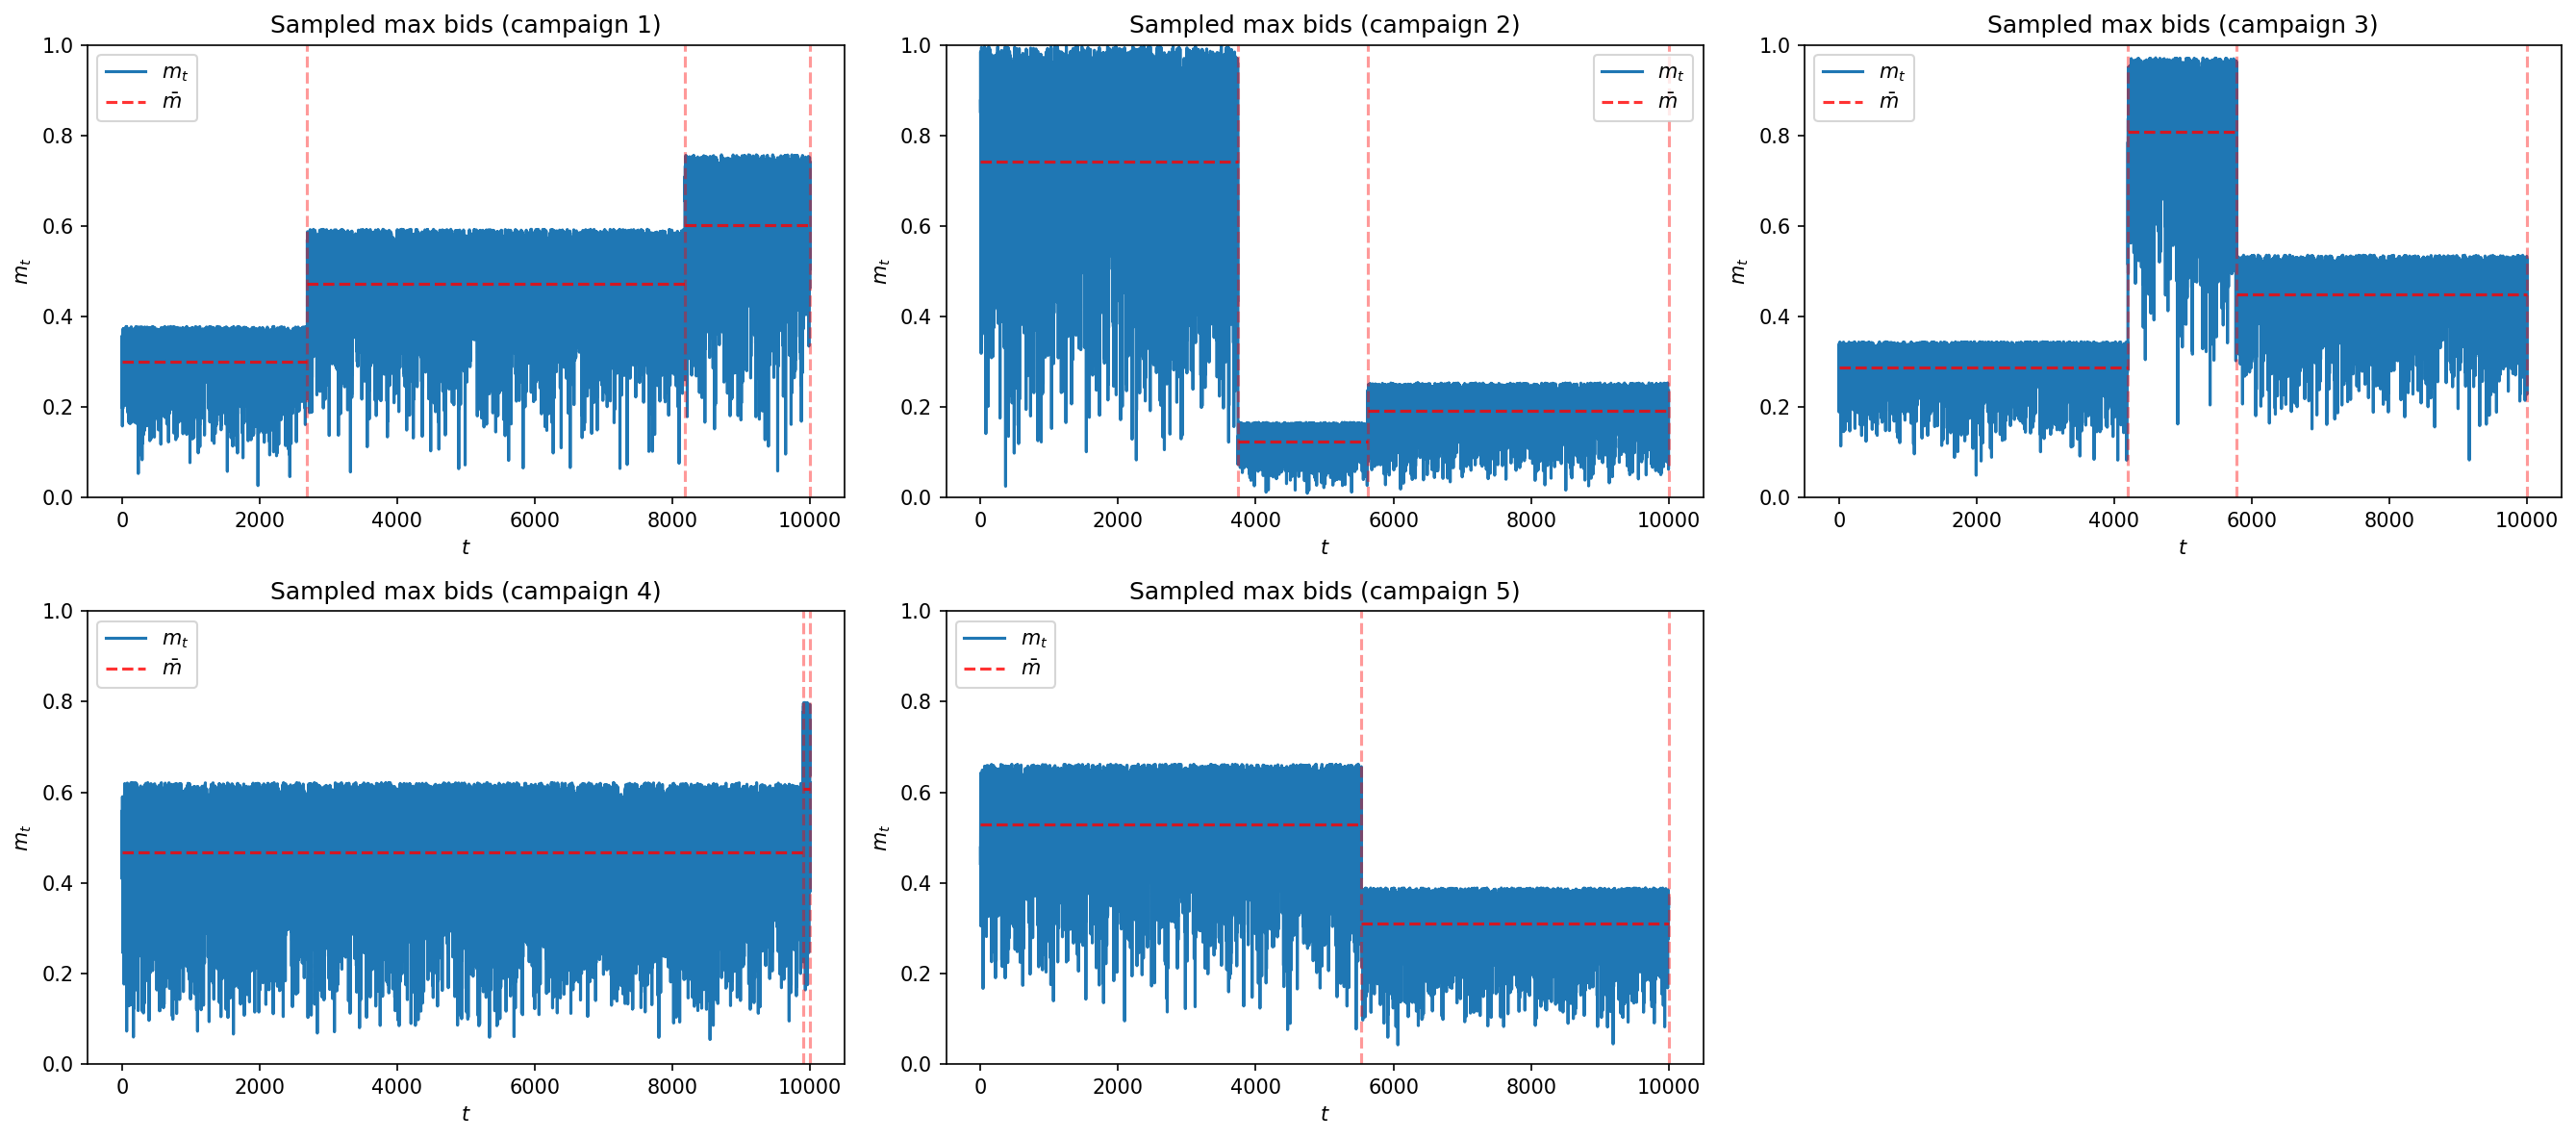
\includegraphics[width=0.7\textwidth]{figures/req4_max_bids_ts_with_changes.png}

    \vspace{-0.1cm}

    \footnotesize\begin{itemize}
        \item For each campaign $i$, independently sample the number of phases $\Upsilon_i \sim \mathrm{Unif}\{2, 3\}$ and then $\Upsilon_i-1$ change times uniformly in $[1,T]$
        
        \vspace{-0.1cm}
        
        \item Each phase has a different upper bound $u^{(i)}_p \sim \mathrm{Unif}(0, 1)$ on competitors' uniform bids
        
        \vspace{-0.1cm}
        
        \item Within a phase: competing bids $\sim \mathrm{Unif}(0, u^{(i)}_p)$, thus $m_p^{(i)} \sim \mathrm{Beta}(n_i,1)$ but \emph{rescaled by $u^{(i)}_p$} 

        \vspace{-0.05cm}

        $\implies$ closed-form win probabilities $\implies$ we \emph{can} write the same LP of the stochastic setting, per-phase
    \end{itemize}
\end{frame}

% ============================================================
% Clairvoyant LP -- piecewise stationary
% ============================================================
\begin{frame}{Clairvoyant: realistic baseline}
    \begin{itemize}
        \item Slightly non-stationary clairvoyant: the one implementing the \emph{best policy} in hindsight (defined in the exercise session)
        \item Actual best policy in a budget-constrained environment: deliberately do not bid at all in some phases, wait for later phases in which highest competing bids are lower instead.
        \item $\implies$ Completely unrealistic: no learner can foresee that a more favourable phase than the current one is coming in the future! 
        \begin{itemize}
            \item (See proof of lower bound for adversarial environment in the course slides)
        \end{itemize}
        \item Thus, we choose the clairvoyant \textbf{not as knowing all the changes in the highest competing bids in advance}, but \textbf{as being able to detect the changes instantaneously as they happen}
        \begin{itemize}
            \item In line with our learners: they "lose rounds" in detecting changes, or in trying to forget the past, or in adjusting against them
        \end{itemize}
    \end{itemize}
\end{frame}

\begin{frame}{Clairvoyant: a per-phase LP on each interval}
    Intersect the phases of all campaigns together and split rounds in a single \emph{joint} partition

    \vspace{0.2cm}

    \begin{block}{}
        A clairvoyant simply needs to solve a stationary LP for each phase in this joint partitioning!
        
        $\implies$ For each joint phase $p$: solve the same clairvoyant LP as in Requirement 2, with phase-specific win probabilities $\mathbb{P}^{(i)}_p(b \ge m)$
    \end{block}

    \vspace{0.8cm}

    \begin{alertblock}{Note:}
        $\rho$ stays the same across phases, it does not get updated!
    \end{alertblock}
\end{frame}


\begin{frame}{Clairvoyant: phase-wise $\gamma_s^\star$ over campaigns subsets}
    \centering
    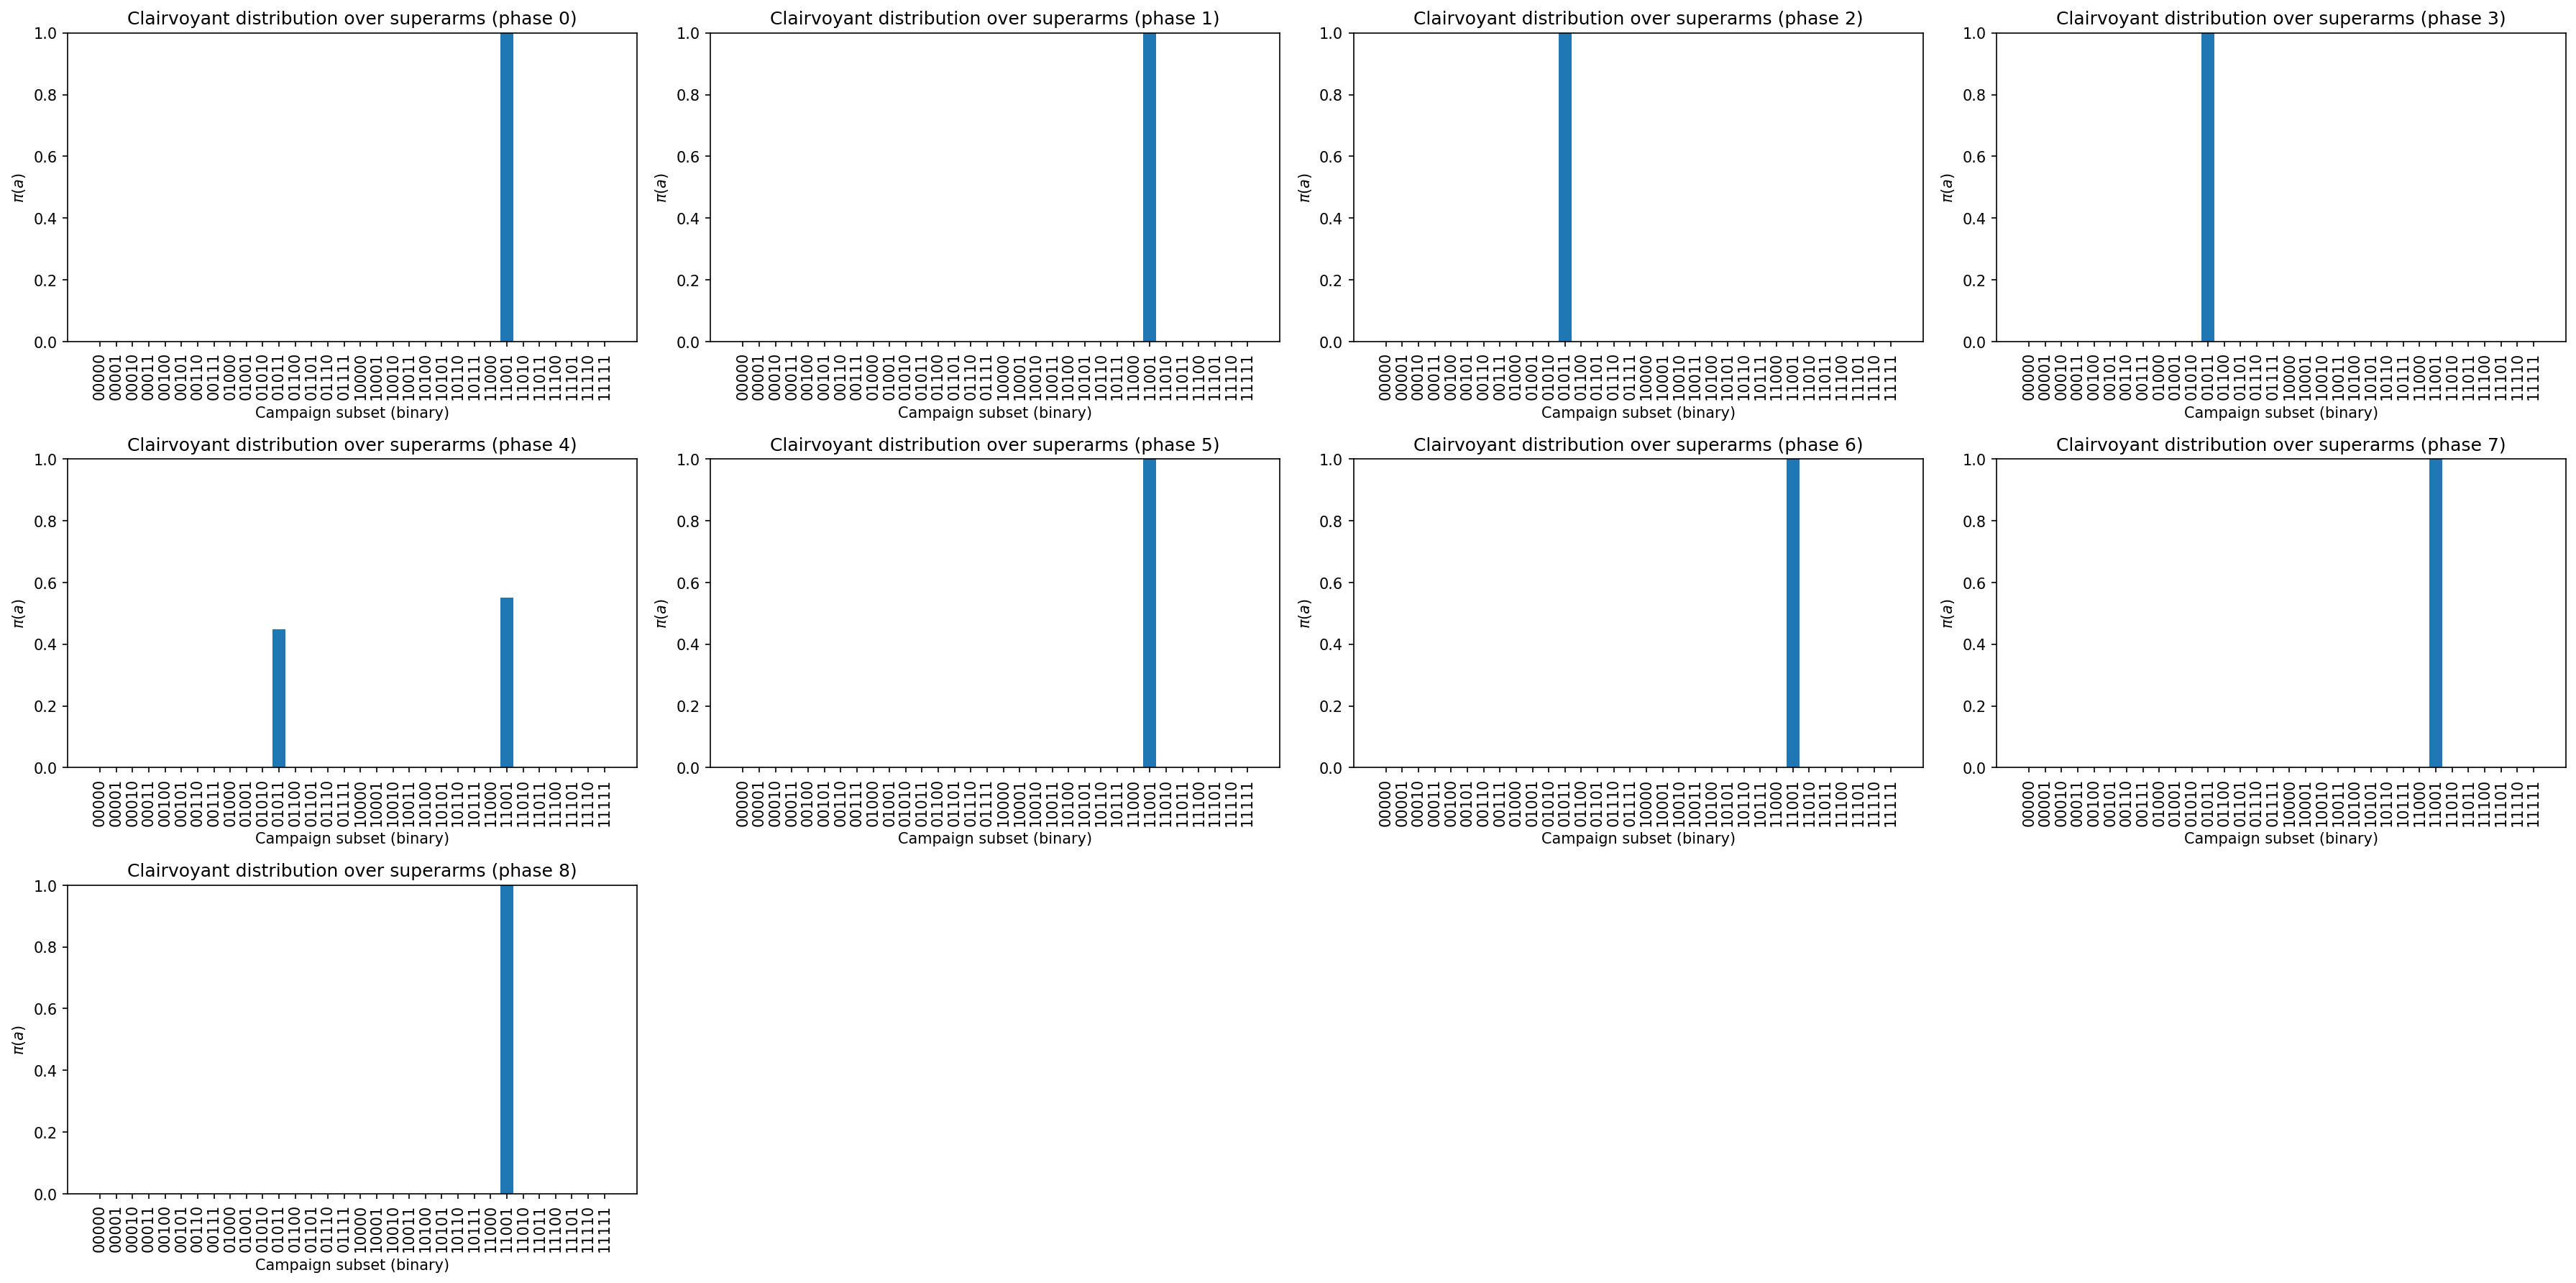
\includegraphics[width=0.8\textwidth]{figures/req4_clairvoyant_gamma_phases.png}\\
    \scriptsize
    Each phase has its own randomization policy over the subsets of campaigns: the policy changes because some campaigns become better/worse in different phases due to the competing bids being non-stationary.
\end{frame}

% ============================================================
% Sliding-window bidder
% ============================================================
\begin{frame}{Sliding-Window Combinatorial-UCB: recap}
    \begin{itemize}
        \item Maintain a \emph{window} of the samples played over the last $\tau$ rounds and the corresponding utilities/costs observed
        \item Confidence radius is computed on the window only: $r(b) = \sqrt{\frac{2 \log \tau}{N_\tau(b)}}$
        \item Theoretically optimal window size: $\tau = \sqrt{\frac{T\log T}{\Upsilon}}$, where $\Upsilon$ is the total amount of (\emph{joint}!) phases
        \begin{itemize}
            \item for unknown $\Upsilon$, set $\Upsilon = T \implies \tau = \sqrt{\log T}$
            \item $\tau \approx \sqrt{T}$ is also a good choice in practice: this is what we use
            \item we actually use $\tau \approx \sqrt{T \log T}$
        \end{itemize}
        
        \item Same underlying bidder as Combinatorial-UCB from Requirement 2
    \end{itemize}
\end{frame}

% ============================================================
% CUSUM bidder
% ============================================================
\begin{frame}{CUSUM Combinatorial-UCB: recap}
    Two phases:
    \begin{itemize}
        \item Estimation phase: build an estimator for the average utility/cost of each arm
        \begin{itemize}
            \item For each campaign, we set an exploration counter to a value $M$, and we keep exploring arms until all the counters reach $0$
            \item We try to select superarms that explore arms that require estimation for multiple campaigns at the same time
            \item At the same time, we do not bid on arms that we have already estimated to avoid wasting budget, since they may no longer be optimal
        \end{itemize}

        \item Detection phase: detect significant deviations from the estimated mean, which signal a phase change
        \begin{itemize}
            \item We compute the positive/negative deviation of the current utility/cost from the estimated means, "dampening" by a quantity $\varepsilon$
            \item We keep track of the positive/negative cumulative deviations from the estimates across multiple rounds
            \item We detect a change if either is larger than a threshold $h$
        \end{itemize}
    \end{itemize}
\end{frame}

\begin{frame}{CUSUM Combinatorial-UCB: recap}
    \begin{itemize}        
        \item Extra probability $\alpha$ of pure exploration per-round to detect changes in arms not being played
        \item Hyperparameters to be tuned: 
        \begin{itemize}
            \item $M$: Length of the estimation phase
            \item $\varepsilon$: "Dampening" factor, how much we expect a sample to deviate from the mean
            \item $h$: Threshold for detecting a change 
            \item $\alpha$: Probability of "pure" exploration per-round  
        \end{itemize}

        \item Again, same underlying bidder as Combinatorial-UCB from Requirement 2
    \end{itemize}
\end{frame}

\begin{frame}{CUSUM in action: detection traces}
    \centering
    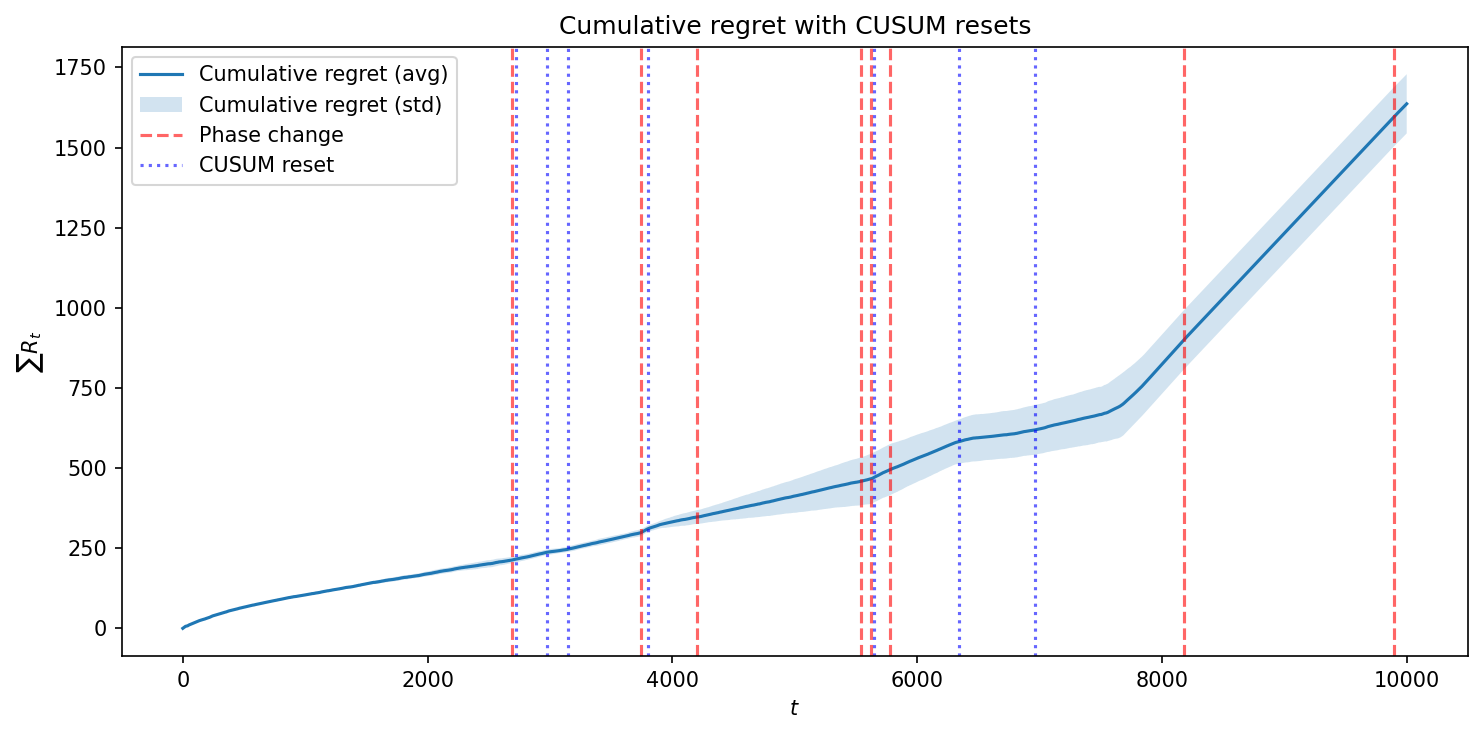
\includegraphics[width=0.75\textwidth]{figures/req4_cusum_resets.png}\\
    \scriptsize
    Joint phase change times (vertical \textcolor{red}{red} lines) and CUSUM reset times (vertical \textcolor{blue}{blue} lines) superimposed on the cumulative-regret curve. Regret can be convex/nonsmooth when changing phase, like the phase change right before round $4000$, or the ones right before round $6000$. A CUSUM reset time can lead to concavity and improvements in the regret, like in the two resets after round $6000$.
\end{frame}

% ============================================================
% Comparison
% ============================================================
\begin{frame}{Comparison: cumulative regret of the bidders}
    \centering
    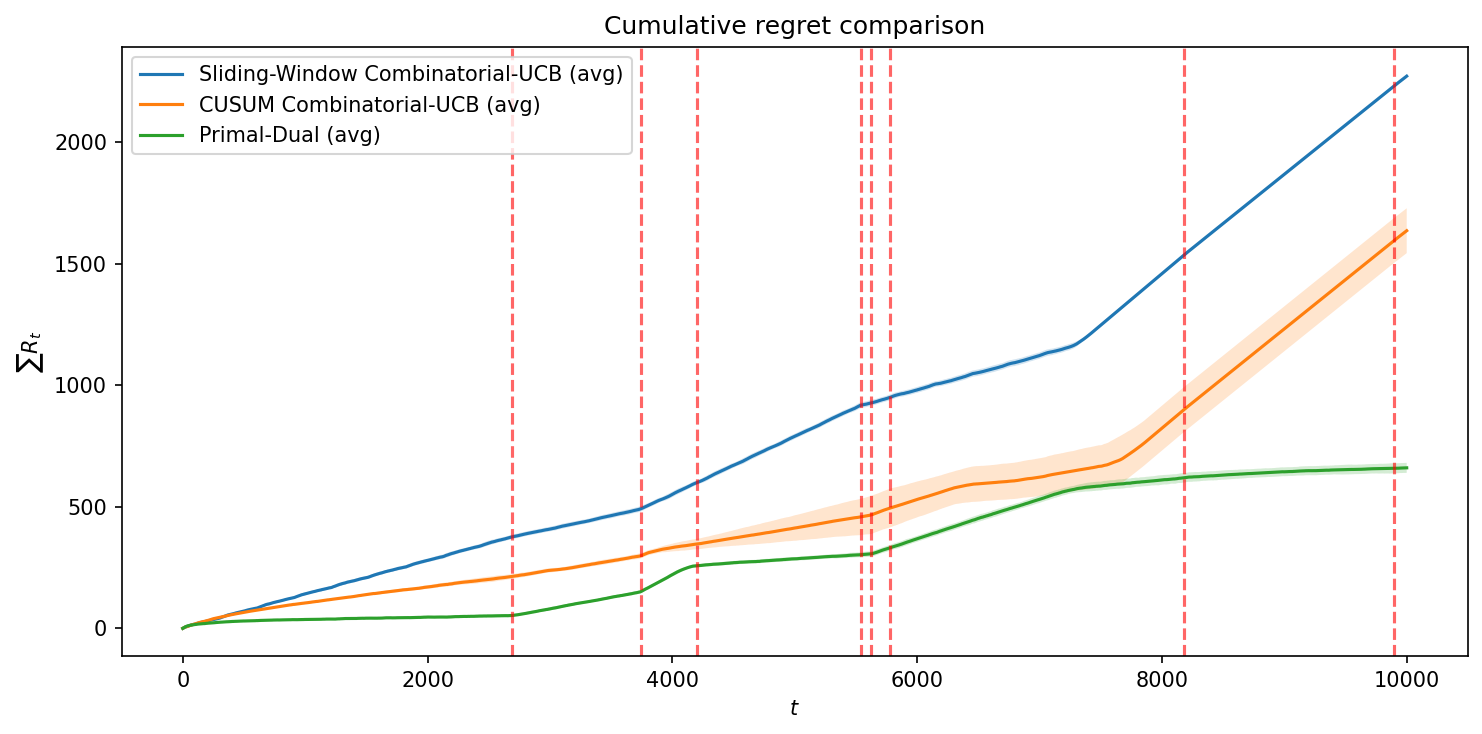
\includegraphics[width=0.75\textwidth]{figures/req4_regret_comparison.png}\\
    \scriptsize
    Unexpectedly, the primal-dual bidder remains the best, with CUSUM Combinatorial-UCB being a surprisingly close second, until it depletes the budget. Sliding-Window Combinatorial-UCB does a bit worse, maybe due to a suboptimal choice of the window size.
    Still, all regrets exhibit sublinear behavior until budget is depleted.
\end{frame}

\section{Recap of the findings}

% ============================================================
% Headline summary
% ============================================================
\begin{frame}{One-slide recap}
    \begin{table}[t]
        \centering
        \small
        \begin{tabular}{l l l l}
            \toprule
            \textbf{Setting} & \textbf{Best fit} & \textbf{Regret} \\
            \midrule
            Stochastic, single campaign & UCB1-like & Sublinear \\
            Stochastic, multi campaign & Combinatorial-UCB & Sublinear$^\star$ \\
            Highly non-stationary      & Primal-dual        & Sublinear \\
            Slightly non-stationary    & CUSUM-UCB          & Sublinear \\
            \bottomrule
        \end{tabular}
    \end{table}
    \centering\scriptsize{$^\star$For Combinatorial-UCB, many more rounds are required, or confidence intervals decaying faster}
    
    \vspace{0.2cm}

    \small\begin{itemize}
        \item \textbf{Clairvoyant} baseline needs to be adapted carefully to the problem, must be neither too strong (unrealistic) nor too weak (non-informative)
        \item \textbf{Hyperparameters} should be tuned carefully, especially for CUSUM and Sliding-Window methods
        \item \textbf{Expensiveness} of the bidder is non-negligible, especially when rounds progress with a fast pace
    \end{itemize}
\end{frame}

% ============================================================
% Closing slide
% ============================================================
\begin{frame}{Thanks!}
    \begin{center}
        \Large
        \emph{Questions?} \\
        \vspace{5mm}
        Code, notebooks and results:   
        \vspace{1cm}
        \small \texttt{https://github.com/Richypiants/online-learning-applications-project-2025-2026/}
    \end{center}
\end{frame}

\end{document}
